% Created by tikzDevice version 0.9 on 2016-03-15 18:17:34
% !TEX encoding = UTF-8 Unicode
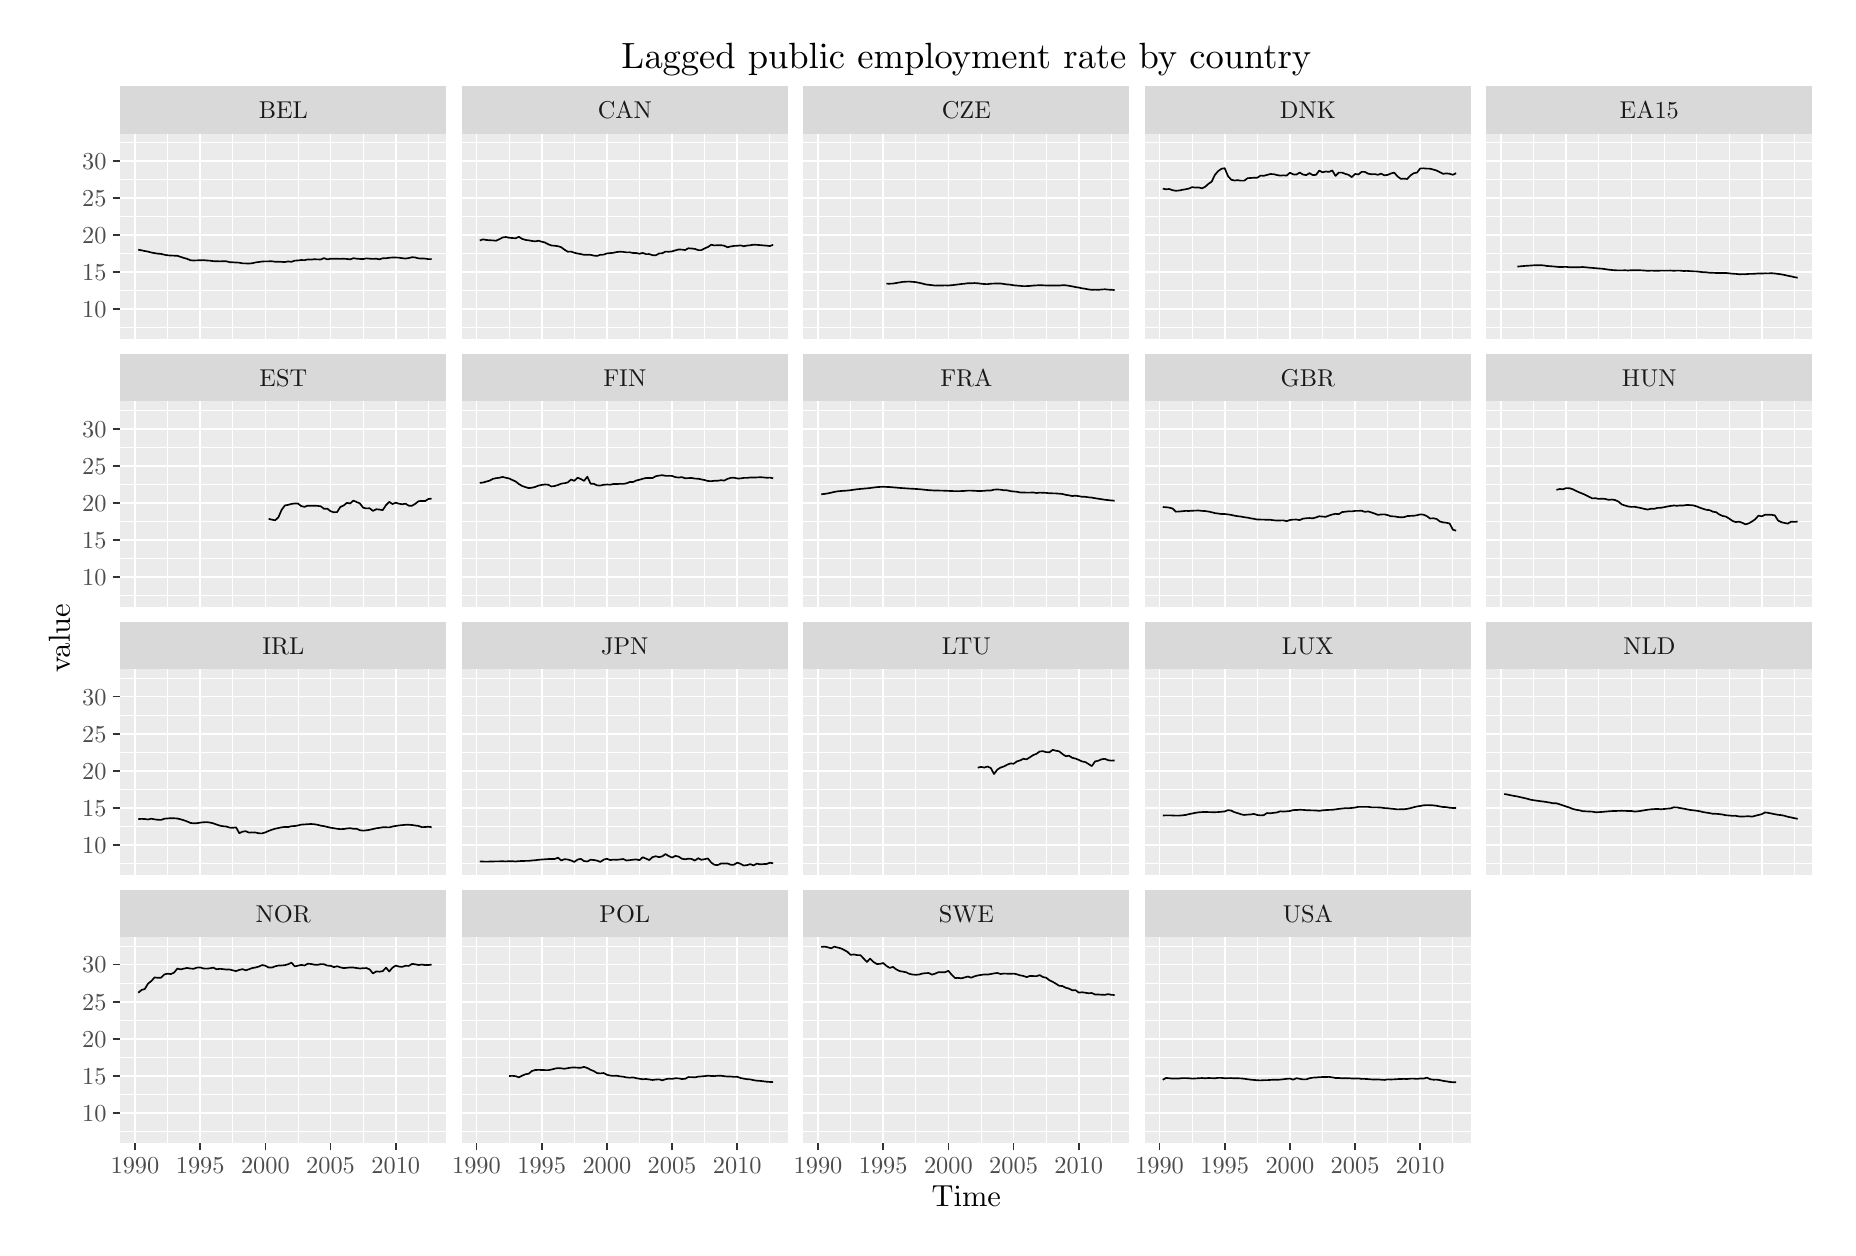
\begin{tikzpicture}[x=1pt,y=1pt]
\definecolor{fillColor}{RGB}{255,255,255}
\path[use as bounding box,fill=fillColor,fill opacity=0.00] (0,0) rectangle (650.43,433.62);
\begin{scope}
\path[clip] (  0.00,  0.00) rectangle (650.43,433.62);
\definecolor{drawColor}{RGB}{255,255,255}
\definecolor{fillColor}{RGB}{255,255,255}

\path[draw=drawColor,line width= 0.6pt,line join=round,line cap=round,fill=fillColor] (  0.00,  0.00) rectangle (650.43,433.62);
\end{scope}
\begin{scope}
\path[clip] ( 33.42,321.12) rectangle (151.33,395.37);
\definecolor{fillColor}{gray}{0.92}

\path[fill=fillColor] ( 33.42,321.12) rectangle (151.33,395.37);
\definecolor{drawColor}{RGB}{255,255,255}

\path[draw=drawColor,line width= 0.3pt,line join=round] ( 33.42,325.16) --
	(151.33,325.16);

\path[draw=drawColor,line width= 0.3pt,line join=round] ( 33.42,338.57) --
	(151.33,338.57);

\path[draw=drawColor,line width= 0.3pt,line join=round] ( 33.42,351.98) --
	(151.33,351.98);

\path[draw=drawColor,line width= 0.3pt,line join=round] ( 33.42,365.39) --
	(151.33,365.39);

\path[draw=drawColor,line width= 0.3pt,line join=round] ( 33.42,378.80) --
	(151.33,378.80);

\path[draw=drawColor,line width= 0.3pt,line join=round] ( 33.42,392.21) --
	(151.33,392.21);

\path[draw=drawColor,line width= 0.3pt,line join=round] ( 50.56,321.12) --
	( 50.56,395.37);

\path[draw=drawColor,line width= 0.3pt,line join=round] ( 74.12,321.12) --
	( 74.12,395.37);

\path[draw=drawColor,line width= 0.3pt,line join=round] ( 97.67,321.12) --
	( 97.67,395.37);

\path[draw=drawColor,line width= 0.3pt,line join=round] (121.23,321.12) --
	(121.23,395.37);

\path[draw=drawColor,line width= 0.3pt,line join=round] (144.79,321.12) --
	(144.79,395.37);

\path[draw=drawColor,line width= 0.6pt,line join=round] ( 33.42,331.86) --
	(151.33,331.86);

\path[draw=drawColor,line width= 0.6pt,line join=round] ( 33.42,345.27) --
	(151.33,345.27);

\path[draw=drawColor,line width= 0.6pt,line join=round] ( 33.42,358.69) --
	(151.33,358.69);

\path[draw=drawColor,line width= 0.6pt,line join=round] ( 33.42,372.10) --
	(151.33,372.10);

\path[draw=drawColor,line width= 0.6pt,line join=round] ( 33.42,385.51) --
	(151.33,385.51);

\path[draw=drawColor,line width= 0.6pt,line join=round] ( 38.78,321.12) --
	( 38.78,395.37);

\path[draw=drawColor,line width= 0.6pt,line join=round] ( 62.34,321.12) --
	( 62.34,395.37);

\path[draw=drawColor,line width= 0.6pt,line join=round] ( 85.90,321.12) --
	( 85.90,395.37);

\path[draw=drawColor,line width= 0.6pt,line join=round] (109.45,321.12) --
	(109.45,395.37);

\path[draw=drawColor,line width= 0.6pt,line join=round] (133.01,321.12) --
	(133.01,395.37);
\definecolor{drawColor}{RGB}{0,0,0}

\path[draw=drawColor,line width= 0.6pt,line join=round] ( 39.96,353.39) --
	( 41.14,353.15) --
	( 42.32,352.91) --
	( 43.49,352.69) --
	( 44.67,352.36) --
	( 45.85,352.15) --
	( 47.03,351.95) --
	( 48.21,351.86) --
	( 49.38,351.57) --
	( 50.56,351.36) --
	( 51.74,351.28) --
	( 52.92,351.23) --
	( 54.09,351.18) --
	( 55.27,350.78) --
	( 56.45,350.40) --
	( 57.63,350.08) --
	( 58.81,349.57) --
	( 59.98,349.49) --
	( 61.16,349.54) --
	( 62.34,349.56) --
	( 63.52,349.61) --
	( 64.70,349.49) --
	( 65.87,349.42) --
	( 67.05,349.25) --
	( 68.23,349.21) --
	( 69.41,349.18) --
	( 70.58,349.19) --
	( 71.76,349.22) --
	( 72.94,348.88) --
	( 74.12,348.83) --
	( 75.30,348.76) --
	( 76.47,348.69) --
	( 77.65,348.46) --
	( 78.83,348.43) --
	( 80.01,348.38) --
	( 81.19,348.50) --
	( 82.36,348.79) --
	( 83.54,348.95) --
	( 84.72,349.11) --
	( 85.90,349.18) --
	( 87.07,349.18) --
	( 88.25,349.21) --
	( 89.43,349.04) --
	( 90.61,349.06) --
	( 91.79,348.98) --
	( 92.96,348.94) --
	( 94.14,349.16) --
	( 95.32,349.01) --
	( 96.50,349.42) --
	( 97.67,349.50) --
	( 98.85,349.66) --
	(100.03,349.60) --
	(101.21,349.87) --
	(102.39,349.80) --
	(103.56,349.94) --
	(104.74,349.88) --
	(105.92,349.86) --
	(107.10,350.35) --
	(108.28,349.87) --
	(109.45,350.14) --
	(110.63,350.12) --
	(111.81,350.13) --
	(112.99,350.07) --
	(114.16,350.12) --
	(115.34,350.04) --
	(116.52,349.89) --
	(117.70,350.31) --
	(118.88,350.14) --
	(120.05,350.05) --
	(121.23,350.00) --
	(122.41,350.26) --
	(123.59,350.13) --
	(124.76,350.06) --
	(125.94,350.13) --
	(127.12,349.91) --
	(128.30,350.29) --
	(129.48,350.28) --
	(130.65,350.48) --
	(131.83,350.56) --
	(133.01,350.55) --
	(134.19,350.50) --
	(135.37,350.31) --
	(136.54,350.20) --
	(137.72,350.36) --
	(138.90,350.68) --
	(140.08,350.57) --
	(141.25,350.24) --
	(142.43,350.22) --
	(143.61,350.17) --
	(144.79,349.98) --
	(145.97,350.00);
\end{scope}
\begin{scope}
\path[clip] (156.83,321.12) rectangle (274.73,395.37);
\definecolor{fillColor}{gray}{0.92}

\path[fill=fillColor] (156.83,321.12) rectangle (274.73,395.37);
\definecolor{drawColor}{RGB}{255,255,255}

\path[draw=drawColor,line width= 0.3pt,line join=round] (156.83,325.16) --
	(274.73,325.16);

\path[draw=drawColor,line width= 0.3pt,line join=round] (156.83,338.57) --
	(274.73,338.57);

\path[draw=drawColor,line width= 0.3pt,line join=round] (156.83,351.98) --
	(274.73,351.98);

\path[draw=drawColor,line width= 0.3pt,line join=round] (156.83,365.39) --
	(274.73,365.39);

\path[draw=drawColor,line width= 0.3pt,line join=round] (156.83,378.80) --
	(274.73,378.80);

\path[draw=drawColor,line width= 0.3pt,line join=round] (156.83,392.21) --
	(274.73,392.21);

\path[draw=drawColor,line width= 0.3pt,line join=round] (173.96,321.12) --
	(173.96,395.37);

\path[draw=drawColor,line width= 0.3pt,line join=round] (197.52,321.12) --
	(197.52,395.37);

\path[draw=drawColor,line width= 0.3pt,line join=round] (221.08,321.12) --
	(221.08,395.37);

\path[draw=drawColor,line width= 0.3pt,line join=round] (244.63,321.12) --
	(244.63,395.37);

\path[draw=drawColor,line width= 0.3pt,line join=round] (268.19,321.12) --
	(268.19,395.37);

\path[draw=drawColor,line width= 0.6pt,line join=round] (156.83,331.86) --
	(274.73,331.86);

\path[draw=drawColor,line width= 0.6pt,line join=round] (156.83,345.27) --
	(274.73,345.27);

\path[draw=drawColor,line width= 0.6pt,line join=round] (156.83,358.69) --
	(274.73,358.69);

\path[draw=drawColor,line width= 0.6pt,line join=round] (156.83,372.10) --
	(274.73,372.10);

\path[draw=drawColor,line width= 0.6pt,line join=round] (156.83,385.51) --
	(274.73,385.51);

\path[draw=drawColor,line width= 0.6pt,line join=round] (162.18,321.12) --
	(162.18,395.37);

\path[draw=drawColor,line width= 0.6pt,line join=round] (185.74,321.12) --
	(185.74,395.37);

\path[draw=drawColor,line width= 0.6pt,line join=round] (209.30,321.12) --
	(209.30,395.37);

\path[draw=drawColor,line width= 0.6pt,line join=round] (232.85,321.12) --
	(232.85,395.37);

\path[draw=drawColor,line width= 0.6pt,line join=round] (256.41,321.12) --
	(256.41,395.37);
\definecolor{drawColor}{RGB}{0,0,0}

\path[draw=drawColor,line width= 0.6pt,line join=round] (163.36,356.71) --
	(164.54,357.13) --
	(165.72,356.90) --
	(166.90,356.80) --
	(168.07,356.75) --
	(169.25,356.63) --
	(170.43,357.18) --
	(171.61,357.80) --
	(172.78,357.98) --
	(173.96,357.71) --
	(175.14,357.60) --
	(176.32,357.52) --
	(177.50,358.04) --
	(178.67,357.31) --
	(179.85,356.92) --
	(181.03,356.77) --
	(182.21,356.55) --
	(183.39,356.39) --
	(184.56,356.62) --
	(185.74,356.28) --
	(186.92,355.98) --
	(188.10,355.35) --
	(189.27,354.90) --
	(190.45,354.81) --
	(191.63,354.64) --
	(192.81,354.28) --
	(193.99,353.38) --
	(195.16,352.66) --
	(196.34,352.71) --
	(197.52,352.31) --
	(198.70,352.00) --
	(199.87,351.81) --
	(201.05,351.53) --
	(202.23,351.55) --
	(203.41,351.53) --
	(204.59,351.25) --
	(205.76,351.13) --
	(206.94,351.57) --
	(208.12,351.60) --
	(209.30,352.05) --
	(210.48,352.16) --
	(211.65,352.27) --
	(212.83,352.54) --
	(214.01,352.66) --
	(215.19,352.59) --
	(216.36,352.41) --
	(217.54,352.44) --
	(218.72,352.20) --
	(219.90,352.18) --
	(221.08,351.92) --
	(222.25,352.23) --
	(223.43,351.78) --
	(224.61,351.81) --
	(225.79,351.41) --
	(226.97,351.35) --
	(228.14,352.02) --
	(229.32,352.10) --
	(230.50,352.69) --
	(231.68,352.66) --
	(232.85,352.77) --
	(234.03,353.15) --
	(235.21,353.46) --
	(236.39,353.42) --
	(237.57,353.26) --
	(238.74,353.90) --
	(239.92,353.82) --
	(241.10,353.67) --
	(242.28,353.24) --
	(243.45,353.23) --
	(244.63,353.86) --
	(245.81,354.36) --
	(246.99,355.18) --
	(248.17,354.93) --
	(249.34,355.01) --
	(250.52,355.02) --
	(251.70,354.82) --
	(252.88,354.28) --
	(254.06,354.56) --
	(255.23,354.75) --
	(256.41,354.81) --
	(257.59,354.95) --
	(258.77,354.64) --
	(259.94,354.88) --
	(261.12,354.99) --
	(262.30,355.20) --
	(263.48,355.14) --
	(264.66,355.04) --
	(265.83,354.94) --
	(267.01,354.84) --
	(268.19,354.71) --
	(269.37,355.16);
\end{scope}
\begin{scope}
\path[clip] (280.23,321.12) rectangle (398.13,395.37);
\definecolor{fillColor}{gray}{0.92}

\path[fill=fillColor] (280.23,321.12) rectangle (398.13,395.37);
\definecolor{drawColor}{RGB}{255,255,255}

\path[draw=drawColor,line width= 0.3pt,line join=round] (280.23,325.16) --
	(398.13,325.16);

\path[draw=drawColor,line width= 0.3pt,line join=round] (280.23,338.57) --
	(398.13,338.57);

\path[draw=drawColor,line width= 0.3pt,line join=round] (280.23,351.98) --
	(398.13,351.98);

\path[draw=drawColor,line width= 0.3pt,line join=round] (280.23,365.39) --
	(398.13,365.39);

\path[draw=drawColor,line width= 0.3pt,line join=round] (280.23,378.80) --
	(398.13,378.80);

\path[draw=drawColor,line width= 0.3pt,line join=round] (280.23,392.21) --
	(398.13,392.21);

\path[draw=drawColor,line width= 0.3pt,line join=round] (297.36,321.12) --
	(297.36,395.37);

\path[draw=drawColor,line width= 0.3pt,line join=round] (320.92,321.12) --
	(320.92,395.37);

\path[draw=drawColor,line width= 0.3pt,line join=round] (344.48,321.12) --
	(344.48,395.37);

\path[draw=drawColor,line width= 0.3pt,line join=round] (368.03,321.12) --
	(368.03,395.37);

\path[draw=drawColor,line width= 0.3pt,line join=round] (391.59,321.12) --
	(391.59,395.37);

\path[draw=drawColor,line width= 0.6pt,line join=round] (280.23,331.86) --
	(398.13,331.86);

\path[draw=drawColor,line width= 0.6pt,line join=round] (280.23,345.27) --
	(398.13,345.27);

\path[draw=drawColor,line width= 0.6pt,line join=round] (280.23,358.69) --
	(398.13,358.69);

\path[draw=drawColor,line width= 0.6pt,line join=round] (280.23,372.10) --
	(398.13,372.10);

\path[draw=drawColor,line width= 0.6pt,line join=round] (280.23,385.51) --
	(398.13,385.51);

\path[draw=drawColor,line width= 0.6pt,line join=round] (285.59,321.12) --
	(285.59,395.37);

\path[draw=drawColor,line width= 0.6pt,line join=round] (309.14,321.12) --
	(309.14,395.37);

\path[draw=drawColor,line width= 0.6pt,line join=round] (332.70,321.12) --
	(332.70,395.37);

\path[draw=drawColor,line width= 0.6pt,line join=round] (356.26,321.12) --
	(356.26,395.37);

\path[draw=drawColor,line width= 0.6pt,line join=round] (379.81,321.12) --
	(379.81,395.37);
\definecolor{drawColor}{RGB}{0,0,0}

\path[draw=drawColor,line width= 0.6pt,line join=round] (310.32,341.12) --
	(311.50,341.10) --
	(312.68,341.15) --
	(313.85,341.35) --
	(315.03,341.56) --
	(316.21,341.75) --
	(317.39,341.83) --
	(318.56,341.87) --
	(319.74,341.77) --
	(320.92,341.66) --
	(322.10,341.43) --
	(323.28,341.16) --
	(324.45,340.84) --
	(325.63,340.69) --
	(326.81,340.57) --
	(327.99,340.41) --
	(329.17,340.48) --
	(330.34,340.46) --
	(331.52,340.49) --
	(332.70,340.46) --
	(333.88,340.55) --
	(335.05,340.69) --
	(336.23,340.84) --
	(337.41,341.00) --
	(338.59,341.11) --
	(339.77,341.28) --
	(340.94,341.26) --
	(342.12,341.33) --
	(343.30,341.26) --
	(344.48,341.09) --
	(345.66,340.98) --
	(346.83,340.94) --
	(348.01,341.10) --
	(349.19,341.14) --
	(350.37,341.20) --
	(351.54,341.17) --
	(352.72,341.01) --
	(353.90,340.83) --
	(355.08,340.74) --
	(356.26,340.53) --
	(357.43,340.42) --
	(358.61,340.33) --
	(359.79,340.21) --
	(360.97,340.24) --
	(362.14,340.30) --
	(363.32,340.42) --
	(364.50,340.50) --
	(365.68,340.54) --
	(366.86,340.52) --
	(368.03,340.46) --
	(369.21,340.44) --
	(370.39,340.45) --
	(371.57,340.44) --
	(372.75,340.44) --
	(373.92,340.54) --
	(375.10,340.52) --
	(376.28,340.34) --
	(377.46,340.13) --
	(378.63,339.88) --
	(379.81,339.70) --
	(380.99,339.43) --
	(382.17,339.27) --
	(383.35,339.03) --
	(384.52,338.90) --
	(385.70,338.95) --
	(386.88,338.90) --
	(388.06,339.00) --
	(389.23,339.08) --
	(390.41,338.96) --
	(391.59,338.91) --
	(392.77,338.81);
\end{scope}
\begin{scope}
\path[clip] (403.63,321.12) rectangle (521.53,395.37);
\definecolor{fillColor}{gray}{0.92}

\path[fill=fillColor] (403.63,321.12) rectangle (521.53,395.37);
\definecolor{drawColor}{RGB}{255,255,255}

\path[draw=drawColor,line width= 0.3pt,line join=round] (403.63,325.16) --
	(521.53,325.16);

\path[draw=drawColor,line width= 0.3pt,line join=round] (403.63,338.57) --
	(521.53,338.57);

\path[draw=drawColor,line width= 0.3pt,line join=round] (403.63,351.98) --
	(521.53,351.98);

\path[draw=drawColor,line width= 0.3pt,line join=round] (403.63,365.39) --
	(521.53,365.39);

\path[draw=drawColor,line width= 0.3pt,line join=round] (403.63,378.80) --
	(521.53,378.80);

\path[draw=drawColor,line width= 0.3pt,line join=round] (403.63,392.21) --
	(521.53,392.21);

\path[draw=drawColor,line width= 0.3pt,line join=round] (420.77,321.12) --
	(420.77,395.37);

\path[draw=drawColor,line width= 0.3pt,line join=round] (444.32,321.12) --
	(444.32,395.37);

\path[draw=drawColor,line width= 0.3pt,line join=round] (467.88,321.12) --
	(467.88,395.37);

\path[draw=drawColor,line width= 0.3pt,line join=round] (491.44,321.12) --
	(491.44,395.37);

\path[draw=drawColor,line width= 0.3pt,line join=round] (514.99,321.12) --
	(514.99,395.37);

\path[draw=drawColor,line width= 0.6pt,line join=round] (403.63,331.86) --
	(521.53,331.86);

\path[draw=drawColor,line width= 0.6pt,line join=round] (403.63,345.27) --
	(521.53,345.27);

\path[draw=drawColor,line width= 0.6pt,line join=round] (403.63,358.69) --
	(521.53,358.69);

\path[draw=drawColor,line width= 0.6pt,line join=round] (403.63,372.10) --
	(521.53,372.10);

\path[draw=drawColor,line width= 0.6pt,line join=round] (403.63,385.51) --
	(521.53,385.51);

\path[draw=drawColor,line width= 0.6pt,line join=round] (408.99,321.12) --
	(408.99,395.37);

\path[draw=drawColor,line width= 0.6pt,line join=round] (432.54,321.12) --
	(432.54,395.37);

\path[draw=drawColor,line width= 0.6pt,line join=round] (456.10,321.12) --
	(456.10,395.37);

\path[draw=drawColor,line width= 0.6pt,line join=round] (479.66,321.12) --
	(479.66,395.37);

\path[draw=drawColor,line width= 0.6pt,line join=round] (503.21,321.12) --
	(503.21,395.37);
\definecolor{drawColor}{RGB}{0,0,0}

\path[draw=drawColor,line width= 0.6pt,line join=round] (410.16,375.44) --
	(411.34,375.22) --
	(412.52,375.32) --
	(413.70,374.88) --
	(414.88,374.68) --
	(416.05,374.77) --
	(417.23,375.02) --
	(418.41,375.23) --
	(419.59,375.47) --
	(420.77,376.00) --
	(421.94,375.82) --
	(423.12,375.90) --
	(424.30,375.56) --
	(425.48,376.10) --
	(426.65,377.17) --
	(427.83,377.97) --
	(429.01,380.44) --
	(430.19,381.80) --
	(431.37,382.63) --
	(432.54,382.84) --
	(433.72,379.99) --
	(434.90,378.67) --
	(436.08,378.40) --
	(437.25,378.51) --
	(438.43,378.33) --
	(439.61,378.33) --
	(440.79,379.22) --
	(441.97,379.31) --
	(443.14,379.39) --
	(444.32,379.40) --
	(445.50,380.17) --
	(446.68,380.09) --
	(447.86,380.42) --
	(449.03,380.73) --
	(450.21,380.68) --
	(451.39,380.38) --
	(452.57,380.15) --
	(453.74,380.26) --
	(454.92,380.17) --
	(456.10,381.19) --
	(457.28,380.60) --
	(458.46,380.52) --
	(459.63,381.28) --
	(460.81,380.55) --
	(461.99,380.32) --
	(463.17,381.05) --
	(464.34,380.36) --
	(465.52,380.42) --
	(466.70,381.96) --
	(467.88,381.36) --
	(469.06,381.64) --
	(470.23,381.50) --
	(471.41,382.02) --
	(472.59,380.05) --
	(473.77,381.25) --
	(474.95,381.24) --
	(476.12,380.80) --
	(477.30,380.43) --
	(478.48,379.62) --
	(479.66,380.76) --
	(480.83,380.57) --
	(482.01,381.50) --
	(483.19,381.51) --
	(484.37,380.85) --
	(485.55,380.66) --
	(486.72,380.71) --
	(487.90,380.46) --
	(489.08,380.87) --
	(490.26,380.26) --
	(491.44,380.42) --
	(492.61,380.94) --
	(493.79,381.25) --
	(494.97,379.89) --
	(496.15,379.01) --
	(497.32,379.06) --
	(498.50,378.94) --
	(499.68,380.23) --
	(500.86,381.02) --
	(502.04,381.25) --
	(503.21,382.77) --
	(504.39,382.79) --
	(505.57,382.68) --
	(506.75,382.66) --
	(507.92,382.34) --
	(509.10,382.00) --
	(510.28,381.40) --
	(511.46,380.79) --
	(512.64,380.97) --
	(513.81,380.81) --
	(514.99,380.47) --
	(516.17,381.02);
\end{scope}
\begin{scope}
\path[clip] (527.03,321.12) rectangle (644.93,395.37);
\definecolor{fillColor}{gray}{0.92}

\path[fill=fillColor] (527.03,321.12) rectangle (644.93,395.37);
\definecolor{drawColor}{RGB}{255,255,255}

\path[draw=drawColor,line width= 0.3pt,line join=round] (527.03,325.16) --
	(644.93,325.16);

\path[draw=drawColor,line width= 0.3pt,line join=round] (527.03,338.57) --
	(644.93,338.57);

\path[draw=drawColor,line width= 0.3pt,line join=round] (527.03,351.98) --
	(644.93,351.98);

\path[draw=drawColor,line width= 0.3pt,line join=round] (527.03,365.39) --
	(644.93,365.39);

\path[draw=drawColor,line width= 0.3pt,line join=round] (527.03,378.80) --
	(644.93,378.80);

\path[draw=drawColor,line width= 0.3pt,line join=round] (527.03,392.21) --
	(644.93,392.21);

\path[draw=drawColor,line width= 0.3pt,line join=round] (544.17,321.12) --
	(544.17,395.37);

\path[draw=drawColor,line width= 0.3pt,line join=round] (567.72,321.12) --
	(567.72,395.37);

\path[draw=drawColor,line width= 0.3pt,line join=round] (591.28,321.12) --
	(591.28,395.37);

\path[draw=drawColor,line width= 0.3pt,line join=round] (614.84,321.12) --
	(614.84,395.37);

\path[draw=drawColor,line width= 0.3pt,line join=round] (638.39,321.12) --
	(638.39,395.37);

\path[draw=drawColor,line width= 0.6pt,line join=round] (527.03,331.86) --
	(644.93,331.86);

\path[draw=drawColor,line width= 0.6pt,line join=round] (527.03,345.27) --
	(644.93,345.27);

\path[draw=drawColor,line width= 0.6pt,line join=round] (527.03,358.69) --
	(644.93,358.69);

\path[draw=drawColor,line width= 0.6pt,line join=round] (527.03,372.10) --
	(644.93,372.10);

\path[draw=drawColor,line width= 0.6pt,line join=round] (527.03,385.51) --
	(644.93,385.51);

\path[draw=drawColor,line width= 0.6pt,line join=round] (532.39,321.12) --
	(532.39,395.37);

\path[draw=drawColor,line width= 0.6pt,line join=round] (555.94,321.12) --
	(555.94,395.37);

\path[draw=drawColor,line width= 0.6pt,line join=round] (579.50,321.12) --
	(579.50,395.37);

\path[draw=drawColor,line width= 0.6pt,line join=round] (603.06,321.12) --
	(603.06,395.37);

\path[draw=drawColor,line width= 0.6pt,line join=round] (626.61,321.12) --
	(626.61,395.37);
\definecolor{drawColor}{RGB}{0,0,0}

\path[draw=drawColor,line width= 0.6pt,line join=round] (538.28,347.30) --
	(539.45,347.38) --
	(540.63,347.50) --
	(541.81,347.58) --
	(542.99,347.66) --
	(544.17,347.74) --
	(545.34,347.75) --
	(546.52,347.80) --
	(547.70,347.72) --
	(548.88,347.52) --
	(550.06,347.43) --
	(551.23,347.35) --
	(552.41,347.22) --
	(553.59,347.13) --
	(554.77,347.16) --
	(555.94,347.18) --
	(557.12,347.05) --
	(558.30,347.06) --
	(559.48,347.03) --
	(560.66,347.05) --
	(561.83,347.13) --
	(563.01,347.03) --
	(564.19,346.90) --
	(565.37,346.81) --
	(566.55,346.71) --
	(567.72,346.59) --
	(568.90,346.52) --
	(570.08,346.36) --
	(571.26,346.17) --
	(572.43,346.05) --
	(573.61,345.94) --
	(574.79,345.92) --
	(575.97,345.90) --
	(577.15,345.95) --
	(578.32,345.88) --
	(579.50,345.97) --
	(580.68,345.98) --
	(581.86,345.97) --
	(583.03,345.93) --
	(584.21,345.86) --
	(585.39,345.75) --
	(586.57,345.82) --
	(587.75,345.80) --
	(588.92,345.76) --
	(590.10,345.83) --
	(591.28,345.81) --
	(592.46,345.81) --
	(593.64,345.85) --
	(594.81,345.78) --
	(595.99,345.83) --
	(597.17,345.81) --
	(598.35,345.70) --
	(599.52,345.73) --
	(600.70,345.65) --
	(601.88,345.57) --
	(603.06,345.54) --
	(604.24,345.39) --
	(605.41,345.27) --
	(606.59,345.22) --
	(607.77,345.05) --
	(608.95,345.03) --
	(610.12,344.98) --
	(611.30,344.94) --
	(612.48,344.96) --
	(613.66,344.99) --
	(614.84,344.84) --
	(616.01,344.72) --
	(617.19,344.65) --
	(618.37,344.52) --
	(619.55,344.55) --
	(620.73,344.54) --
	(621.90,344.64) --
	(623.08,344.65) --
	(624.26,344.71) --
	(625.44,344.82) --
	(626.61,344.77) --
	(627.79,344.85) --
	(628.97,344.83) --
	(630.15,344.88) --
	(631.33,344.79) --
	(632.50,344.64) --
	(633.68,344.49) --
	(634.86,344.24) --
	(636.04,343.97) --
	(637.22,343.75) --
	(638.39,343.47) --
	(639.57,343.25);
\end{scope}
\begin{scope}
\path[clip] ( 33.42,224.31) rectangle (151.33,298.56);
\definecolor{fillColor}{gray}{0.92}

\path[fill=fillColor] ( 33.42,224.31) rectangle (151.33,298.56);
\definecolor{drawColor}{RGB}{255,255,255}

\path[draw=drawColor,line width= 0.3pt,line join=round] ( 33.42,228.35) --
	(151.33,228.35);

\path[draw=drawColor,line width= 0.3pt,line join=round] ( 33.42,241.76) --
	(151.33,241.76);

\path[draw=drawColor,line width= 0.3pt,line join=round] ( 33.42,255.17) --
	(151.33,255.17);

\path[draw=drawColor,line width= 0.3pt,line join=round] ( 33.42,268.58) --
	(151.33,268.58);

\path[draw=drawColor,line width= 0.3pt,line join=round] ( 33.42,281.99) --
	(151.33,281.99);

\path[draw=drawColor,line width= 0.3pt,line join=round] ( 33.42,295.40) --
	(151.33,295.40);

\path[draw=drawColor,line width= 0.3pt,line join=round] ( 50.56,224.31) --
	( 50.56,298.56);

\path[draw=drawColor,line width= 0.3pt,line join=round] ( 74.12,224.31) --
	( 74.12,298.56);

\path[draw=drawColor,line width= 0.3pt,line join=round] ( 97.67,224.31) --
	( 97.67,298.56);

\path[draw=drawColor,line width= 0.3pt,line join=round] (121.23,224.31) --
	(121.23,298.56);

\path[draw=drawColor,line width= 0.3pt,line join=round] (144.79,224.31) --
	(144.79,298.56);

\path[draw=drawColor,line width= 0.6pt,line join=round] ( 33.42,235.05) --
	(151.33,235.05);

\path[draw=drawColor,line width= 0.6pt,line join=round] ( 33.42,248.46) --
	(151.33,248.46);

\path[draw=drawColor,line width= 0.6pt,line join=round] ( 33.42,261.87) --
	(151.33,261.87);

\path[draw=drawColor,line width= 0.6pt,line join=round] ( 33.42,275.29) --
	(151.33,275.29);

\path[draw=drawColor,line width= 0.6pt,line join=round] ( 33.42,288.70) --
	(151.33,288.70);

\path[draw=drawColor,line width= 0.6pt,line join=round] ( 38.78,224.31) --
	( 38.78,298.56);

\path[draw=drawColor,line width= 0.6pt,line join=round] ( 62.34,224.31) --
	( 62.34,298.56);

\path[draw=drawColor,line width= 0.6pt,line join=round] ( 85.90,224.31) --
	( 85.90,298.56);

\path[draw=drawColor,line width= 0.6pt,line join=round] (109.45,224.31) --
	(109.45,298.56);

\path[draw=drawColor,line width= 0.6pt,line join=round] (133.01,224.31) --
	(133.01,298.56);
\definecolor{drawColor}{RGB}{0,0,0}

\path[draw=drawColor,line width= 0.6pt,line join=round] ( 87.07,256.15) --
	( 88.25,255.83) --
	( 89.43,255.60) --
	( 90.61,256.70) --
	( 91.79,259.44) --
	( 92.96,260.97) --
	( 94.14,261.20) --
	( 95.32,261.52) --
	( 96.50,261.69) --
	( 97.67,261.65) --
	( 98.85,260.74) --
	(100.03,260.47) --
	(101.21,260.89) --
	(102.39,260.88) --
	(103.56,260.89) --
	(104.74,260.82) --
	(105.92,260.67) --
	(107.10,259.74) --
	(108.28,259.81) --
	(109.45,258.88) --
	(110.63,258.52) --
	(111.81,258.58) --
	(112.99,260.43) --
	(114.16,260.94) --
	(115.34,261.92) --
	(116.52,261.69) --
	(117.70,262.73) --
	(118.88,262.19) --
	(120.05,261.70) --
	(121.23,260.15) --
	(122.41,259.90) --
	(123.59,259.95) --
	(124.76,259.01) --
	(125.94,259.60) --
	(127.12,259.49) --
	(128.30,259.28) --
	(129.48,261.10) --
	(130.65,262.26) --
	(131.83,261.48) --
	(133.01,261.98) --
	(134.19,261.59) --
	(135.37,261.41) --
	(136.54,261.62) --
	(137.72,260.87) --
	(138.90,260.88) --
	(140.08,261.59) --
	(141.25,262.52) --
	(142.43,262.59) --
	(143.61,262.56) --
	(144.79,263.30) --
	(145.97,263.45);
\end{scope}
\begin{scope}
\path[clip] (156.83,224.31) rectangle (274.73,298.56);
\definecolor{fillColor}{gray}{0.92}

\path[fill=fillColor] (156.83,224.31) rectangle (274.73,298.56);
\definecolor{drawColor}{RGB}{255,255,255}

\path[draw=drawColor,line width= 0.3pt,line join=round] (156.83,228.35) --
	(274.73,228.35);

\path[draw=drawColor,line width= 0.3pt,line join=round] (156.83,241.76) --
	(274.73,241.76);

\path[draw=drawColor,line width= 0.3pt,line join=round] (156.83,255.17) --
	(274.73,255.17);

\path[draw=drawColor,line width= 0.3pt,line join=round] (156.83,268.58) --
	(274.73,268.58);

\path[draw=drawColor,line width= 0.3pt,line join=round] (156.83,281.99) --
	(274.73,281.99);

\path[draw=drawColor,line width= 0.3pt,line join=round] (156.83,295.40) --
	(274.73,295.40);

\path[draw=drawColor,line width= 0.3pt,line join=round] (173.96,224.31) --
	(173.96,298.56);

\path[draw=drawColor,line width= 0.3pt,line join=round] (197.52,224.31) --
	(197.52,298.56);

\path[draw=drawColor,line width= 0.3pt,line join=round] (221.08,224.31) --
	(221.08,298.56);

\path[draw=drawColor,line width= 0.3pt,line join=round] (244.63,224.31) --
	(244.63,298.56);

\path[draw=drawColor,line width= 0.3pt,line join=round] (268.19,224.31) --
	(268.19,298.56);

\path[draw=drawColor,line width= 0.6pt,line join=round] (156.83,235.05) --
	(274.73,235.05);

\path[draw=drawColor,line width= 0.6pt,line join=round] (156.83,248.46) --
	(274.73,248.46);

\path[draw=drawColor,line width= 0.6pt,line join=round] (156.83,261.87) --
	(274.73,261.87);

\path[draw=drawColor,line width= 0.6pt,line join=round] (156.83,275.29) --
	(274.73,275.29);

\path[draw=drawColor,line width= 0.6pt,line join=round] (156.83,288.70) --
	(274.73,288.70);

\path[draw=drawColor,line width= 0.6pt,line join=round] (162.18,224.31) --
	(162.18,298.56);

\path[draw=drawColor,line width= 0.6pt,line join=round] (185.74,224.31) --
	(185.74,298.56);

\path[draw=drawColor,line width= 0.6pt,line join=round] (209.30,224.31) --
	(209.30,298.56);

\path[draw=drawColor,line width= 0.6pt,line join=round] (232.85,224.31) --
	(232.85,298.56);

\path[draw=drawColor,line width= 0.6pt,line join=round] (256.41,224.31) --
	(256.41,298.56);
\definecolor{drawColor}{RGB}{0,0,0}

\path[draw=drawColor,line width= 0.6pt,line join=round] (163.36,269.12) --
	(164.54,269.25) --
	(165.72,269.61) --
	(166.90,269.92) --
	(168.07,270.57) --
	(169.25,270.83) --
	(170.43,270.97) --
	(171.61,271.28) --
	(172.78,270.97) --
	(173.96,270.72) --
	(175.14,270.17) --
	(176.32,269.64) --
	(177.50,268.70) --
	(178.67,268.01) --
	(179.85,267.60) --
	(181.03,267.24) --
	(182.21,267.37) --
	(183.39,267.67) --
	(184.56,268.15) --
	(185.74,268.38) --
	(186.92,268.56) --
	(188.10,268.45) --
	(189.27,267.83) --
	(190.45,268.01) --
	(191.63,268.36) --
	(192.81,268.86) --
	(193.99,269.00) --
	(195.16,269.29) --
	(196.34,270.33) --
	(197.52,269.87) --
	(198.70,271.00) --
	(199.87,270.53) --
	(201.05,269.86) --
	(202.23,271.35) --
	(203.41,268.83) --
	(204.59,268.80) --
	(205.76,268.22) --
	(206.94,268.18) --
	(208.12,268.43) --
	(209.30,268.53) --
	(210.48,268.47) --
	(211.65,268.72) --
	(212.83,268.69) --
	(214.01,268.79) --
	(215.19,268.76) --
	(216.36,268.96) --
	(217.54,269.44) --
	(218.72,269.42) --
	(219.90,270.00) --
	(221.08,270.25) --
	(222.25,270.62) --
	(223.43,270.89) --
	(224.61,270.87) --
	(225.79,270.87) --
	(226.97,271.54) --
	(228.14,271.76) --
	(229.32,271.90) --
	(230.50,271.67) --
	(231.68,271.66) --
	(232.85,271.64) --
	(234.03,271.20) --
	(235.21,271.06) --
	(236.39,271.21) --
	(237.57,270.78) --
	(238.74,270.85) --
	(239.92,270.91) --
	(241.10,270.67) --
	(242.28,270.63) --
	(243.45,270.39) --
	(244.63,270.14) --
	(245.81,269.80) --
	(246.99,269.75) --
	(248.17,269.88) --
	(249.34,269.88) --
	(250.52,270.11) --
	(251.70,269.96) --
	(252.88,270.58) --
	(254.06,270.94) --
	(255.23,270.99) --
	(256.41,270.73) --
	(257.59,270.74) --
	(258.77,270.93) --
	(259.94,270.93) --
	(261.12,271.07) --
	(262.30,271.10) --
	(263.48,271.10) --
	(264.66,271.17) --
	(265.83,271.11) --
	(267.01,270.98) --
	(268.19,271.03) --
	(269.37,270.80);
\end{scope}
\begin{scope}
\path[clip] (280.23,224.31) rectangle (398.13,298.56);
\definecolor{fillColor}{gray}{0.92}

\path[fill=fillColor] (280.23,224.31) rectangle (398.13,298.56);
\definecolor{drawColor}{RGB}{255,255,255}

\path[draw=drawColor,line width= 0.3pt,line join=round] (280.23,228.35) --
	(398.13,228.35);

\path[draw=drawColor,line width= 0.3pt,line join=round] (280.23,241.76) --
	(398.13,241.76);

\path[draw=drawColor,line width= 0.3pt,line join=round] (280.23,255.17) --
	(398.13,255.17);

\path[draw=drawColor,line width= 0.3pt,line join=round] (280.23,268.58) --
	(398.13,268.58);

\path[draw=drawColor,line width= 0.3pt,line join=round] (280.23,281.99) --
	(398.13,281.99);

\path[draw=drawColor,line width= 0.3pt,line join=round] (280.23,295.40) --
	(398.13,295.40);

\path[draw=drawColor,line width= 0.3pt,line join=round] (297.36,224.31) --
	(297.36,298.56);

\path[draw=drawColor,line width= 0.3pt,line join=round] (320.92,224.31) --
	(320.92,298.56);

\path[draw=drawColor,line width= 0.3pt,line join=round] (344.48,224.31) --
	(344.48,298.56);

\path[draw=drawColor,line width= 0.3pt,line join=round] (368.03,224.31) --
	(368.03,298.56);

\path[draw=drawColor,line width= 0.3pt,line join=round] (391.59,224.31) --
	(391.59,298.56);

\path[draw=drawColor,line width= 0.6pt,line join=round] (280.23,235.05) --
	(398.13,235.05);

\path[draw=drawColor,line width= 0.6pt,line join=round] (280.23,248.46) --
	(398.13,248.46);

\path[draw=drawColor,line width= 0.6pt,line join=round] (280.23,261.87) --
	(398.13,261.87);

\path[draw=drawColor,line width= 0.6pt,line join=round] (280.23,275.29) --
	(398.13,275.29);

\path[draw=drawColor,line width= 0.6pt,line join=round] (280.23,288.70) --
	(398.13,288.70);

\path[draw=drawColor,line width= 0.6pt,line join=round] (285.59,224.31) --
	(285.59,298.56);

\path[draw=drawColor,line width= 0.6pt,line join=round] (309.14,224.31) --
	(309.14,298.56);

\path[draw=drawColor,line width= 0.6pt,line join=round] (332.70,224.31) --
	(332.70,298.56);

\path[draw=drawColor,line width= 0.6pt,line join=round] (356.26,224.31) --
	(356.26,298.56);

\path[draw=drawColor,line width= 0.6pt,line join=round] (379.81,224.31) --
	(379.81,298.56);
\definecolor{drawColor}{RGB}{0,0,0}

\path[draw=drawColor,line width= 0.6pt,line join=round] (286.76,265.02) --
	(287.94,265.14) --
	(289.12,265.33) --
	(290.30,265.58) --
	(291.47,265.87) --
	(292.65,266.07) --
	(293.83,266.19) --
	(295.01,266.27) --
	(296.19,266.35) --
	(297.36,266.49) --
	(298.54,266.66) --
	(299.72,266.83) --
	(300.90,266.94) --
	(302.08,267.05) --
	(303.25,267.15) --
	(304.43,267.27) --
	(305.61,267.44) --
	(306.79,267.58) --
	(307.96,267.67) --
	(309.14,267.71) --
	(310.32,267.67) --
	(311.50,267.61) --
	(312.68,267.52) --
	(313.85,267.43) --
	(315.03,267.32) --
	(316.21,267.23) --
	(317.39,267.15) --
	(318.56,267.06) --
	(319.74,267.01) --
	(320.92,266.93) --
	(322.10,266.85) --
	(323.28,266.74) --
	(324.45,266.61) --
	(325.63,266.50) --
	(326.81,266.42) --
	(327.99,266.36) --
	(329.17,266.35) --
	(330.34,266.33) --
	(331.52,266.29) --
	(332.70,266.24) --
	(333.88,266.18) --
	(335.05,266.14) --
	(336.23,266.14) --
	(337.41,266.17) --
	(338.59,266.23) --
	(339.77,266.34) --
	(340.94,266.33) --
	(342.12,266.26) --
	(343.30,266.20) --
	(344.48,266.20) --
	(345.66,266.26) --
	(346.83,266.40) --
	(348.01,266.38) --
	(349.19,266.68) --
	(350.37,266.75) --
	(351.54,266.66) --
	(352.72,266.47) --
	(353.90,266.44) --
	(355.08,266.16) --
	(356.26,266.01) --
	(357.43,265.93) --
	(358.61,265.66) --
	(359.79,265.67) --
	(360.97,265.60) --
	(362.14,265.59) --
	(363.32,265.69) --
	(364.50,265.46) --
	(365.68,265.61) --
	(366.86,265.56) --
	(368.03,265.51) --
	(369.21,265.38) --
	(370.39,265.35) --
	(371.57,265.32) --
	(372.75,265.22) --
	(373.92,265.12) --
	(375.10,264.80) --
	(376.28,264.63) --
	(377.46,264.37) --
	(378.63,264.52) --
	(379.81,264.33) --
	(380.99,264.10) --
	(382.17,264.09) --
	(383.35,263.91) --
	(384.52,263.81) --
	(385.70,263.59) --
	(386.88,263.40) --
	(388.06,263.22) --
	(389.23,263.03) --
	(390.41,262.91) --
	(391.59,262.77) --
	(392.77,262.68);
\end{scope}
\begin{scope}
\path[clip] (403.63,224.31) rectangle (521.53,298.56);
\definecolor{fillColor}{gray}{0.92}

\path[fill=fillColor] (403.63,224.31) rectangle (521.53,298.56);
\definecolor{drawColor}{RGB}{255,255,255}

\path[draw=drawColor,line width= 0.3pt,line join=round] (403.63,228.35) --
	(521.53,228.35);

\path[draw=drawColor,line width= 0.3pt,line join=round] (403.63,241.76) --
	(521.53,241.76);

\path[draw=drawColor,line width= 0.3pt,line join=round] (403.63,255.17) --
	(521.53,255.17);

\path[draw=drawColor,line width= 0.3pt,line join=round] (403.63,268.58) --
	(521.53,268.58);

\path[draw=drawColor,line width= 0.3pt,line join=round] (403.63,281.99) --
	(521.53,281.99);

\path[draw=drawColor,line width= 0.3pt,line join=round] (403.63,295.40) --
	(521.53,295.40);

\path[draw=drawColor,line width= 0.3pt,line join=round] (420.77,224.31) --
	(420.77,298.56);

\path[draw=drawColor,line width= 0.3pt,line join=round] (444.32,224.31) --
	(444.32,298.56);

\path[draw=drawColor,line width= 0.3pt,line join=round] (467.88,224.31) --
	(467.88,298.56);

\path[draw=drawColor,line width= 0.3pt,line join=round] (491.44,224.31) --
	(491.44,298.56);

\path[draw=drawColor,line width= 0.3pt,line join=round] (514.99,224.31) --
	(514.99,298.56);

\path[draw=drawColor,line width= 0.6pt,line join=round] (403.63,235.05) --
	(521.53,235.05);

\path[draw=drawColor,line width= 0.6pt,line join=round] (403.63,248.46) --
	(521.53,248.46);

\path[draw=drawColor,line width= 0.6pt,line join=round] (403.63,261.87) --
	(521.53,261.87);

\path[draw=drawColor,line width= 0.6pt,line join=round] (403.63,275.29) --
	(521.53,275.29);

\path[draw=drawColor,line width= 0.6pt,line join=round] (403.63,288.70) --
	(521.53,288.70);

\path[draw=drawColor,line width= 0.6pt,line join=round] (408.99,224.31) --
	(408.99,298.56);

\path[draw=drawColor,line width= 0.6pt,line join=round] (432.54,224.31) --
	(432.54,298.56);

\path[draw=drawColor,line width= 0.6pt,line join=round] (456.10,224.31) --
	(456.10,298.56);

\path[draw=drawColor,line width= 0.6pt,line join=round] (479.66,224.31) --
	(479.66,298.56);

\path[draw=drawColor,line width= 0.6pt,line join=round] (503.21,224.31) --
	(503.21,298.56);
\definecolor{drawColor}{RGB}{0,0,0}

\path[draw=drawColor,line width= 0.6pt,line join=round] (410.16,260.40) --
	(411.34,260.34) --
	(412.52,260.17) --
	(413.70,259.87) --
	(414.88,258.72) --
	(416.05,258.78) --
	(417.23,258.89) --
	(418.41,259.01) --
	(419.59,258.98) --
	(420.77,259.06) --
	(421.94,259.11) --
	(423.12,259.13) --
	(424.30,259.01) --
	(425.48,258.95) --
	(426.65,258.77) --
	(427.83,258.51) --
	(429.01,258.21) --
	(430.19,258.05) --
	(431.37,257.86) --
	(432.54,257.87) --
	(433.72,257.73) --
	(434.90,257.55) --
	(436.08,257.28) --
	(437.25,257.08) --
	(438.43,256.96) --
	(439.61,256.72) --
	(440.79,256.57) --
	(441.97,256.31) --
	(443.14,256.13) --
	(444.32,255.87) --
	(445.50,255.87) --
	(446.68,255.84) --
	(447.86,255.81) --
	(449.03,255.78) --
	(450.21,255.62) --
	(451.39,255.51) --
	(452.57,255.56) --
	(453.74,255.57) --
	(454.92,255.31) --
	(456.10,255.71) --
	(457.28,255.86) --
	(458.46,255.87) --
	(459.63,255.69) --
	(460.81,256.19) --
	(461.99,256.36) --
	(463.17,256.42) --
	(464.34,256.30) --
	(465.52,256.65) --
	(466.70,257.06) --
	(467.88,256.96) --
	(469.06,256.86) --
	(470.23,257.32) --
	(471.41,257.71) --
	(472.59,257.95) --
	(473.77,257.82) --
	(474.95,258.57) --
	(476.12,258.71) --
	(477.30,258.85) --
	(478.48,258.84) --
	(479.66,259.00) --
	(480.83,259.00) --
	(482.01,259.08) --
	(483.19,258.63) --
	(484.37,258.83) --
	(485.55,258.43) --
	(486.72,258.06) --
	(487.90,257.55) --
	(489.08,257.72) --
	(490.26,257.76) --
	(491.44,257.47) --
	(492.61,257.05) --
	(493.79,257.03) --
	(494.97,256.81) --
	(496.15,256.68) --
	(497.32,256.75) --
	(498.50,257.14) --
	(499.68,257.20) --
	(500.86,257.25) --
	(502.04,257.44) --
	(503.21,257.75) --
	(504.39,257.63) --
	(505.57,257.13) --
	(506.75,256.27) --
	(507.92,256.33) --
	(509.10,256.10) --
	(510.28,255.18) --
	(511.46,254.85) --
	(512.64,254.72) --
	(513.81,254.46) --
	(514.99,252.22) --
	(516.17,251.85);
\end{scope}
\begin{scope}
\path[clip] (527.03,224.31) rectangle (644.93,298.56);
\definecolor{fillColor}{gray}{0.92}

\path[fill=fillColor] (527.03,224.31) rectangle (644.93,298.56);
\definecolor{drawColor}{RGB}{255,255,255}

\path[draw=drawColor,line width= 0.3pt,line join=round] (527.03,228.35) --
	(644.93,228.35);

\path[draw=drawColor,line width= 0.3pt,line join=round] (527.03,241.76) --
	(644.93,241.76);

\path[draw=drawColor,line width= 0.3pt,line join=round] (527.03,255.17) --
	(644.93,255.17);

\path[draw=drawColor,line width= 0.3pt,line join=round] (527.03,268.58) --
	(644.93,268.58);

\path[draw=drawColor,line width= 0.3pt,line join=round] (527.03,281.99) --
	(644.93,281.99);

\path[draw=drawColor,line width= 0.3pt,line join=round] (527.03,295.40) --
	(644.93,295.40);

\path[draw=drawColor,line width= 0.3pt,line join=round] (544.17,224.31) --
	(544.17,298.56);

\path[draw=drawColor,line width= 0.3pt,line join=round] (567.72,224.31) --
	(567.72,298.56);

\path[draw=drawColor,line width= 0.3pt,line join=round] (591.28,224.31) --
	(591.28,298.56);

\path[draw=drawColor,line width= 0.3pt,line join=round] (614.84,224.31) --
	(614.84,298.56);

\path[draw=drawColor,line width= 0.3pt,line join=round] (638.39,224.31) --
	(638.39,298.56);

\path[draw=drawColor,line width= 0.6pt,line join=round] (527.03,235.05) --
	(644.93,235.05);

\path[draw=drawColor,line width= 0.6pt,line join=round] (527.03,248.46) --
	(644.93,248.46);

\path[draw=drawColor,line width= 0.6pt,line join=round] (527.03,261.87) --
	(644.93,261.87);

\path[draw=drawColor,line width= 0.6pt,line join=round] (527.03,275.29) --
	(644.93,275.29);

\path[draw=drawColor,line width= 0.6pt,line join=round] (527.03,288.70) --
	(644.93,288.70);

\path[draw=drawColor,line width= 0.6pt,line join=round] (532.39,224.31) --
	(532.39,298.56);

\path[draw=drawColor,line width= 0.6pt,line join=round] (555.94,224.31) --
	(555.94,298.56);

\path[draw=drawColor,line width= 0.6pt,line join=round] (579.50,224.31) --
	(579.50,298.56);

\path[draw=drawColor,line width= 0.6pt,line join=round] (603.06,224.31) --
	(603.06,298.56);

\path[draw=drawColor,line width= 0.6pt,line join=round] (626.61,224.31) --
	(626.61,298.56);
\definecolor{drawColor}{RGB}{0,0,0}

\path[draw=drawColor,line width= 0.6pt,line join=round] (552.41,266.61) --
	(553.59,266.91) --
	(554.77,266.82) --
	(555.94,267.24) --
	(557.12,267.19) --
	(558.30,266.85) --
	(559.48,266.24) --
	(560.66,265.69) --
	(561.83,265.25) --
	(563.01,264.71) --
	(564.19,264.11) --
	(565.37,263.51) --
	(566.55,263.60) --
	(567.72,263.33) --
	(568.90,263.41) --
	(570.08,263.32) --
	(571.26,262.99) --
	(572.43,263.11) --
	(573.61,262.92) --
	(574.79,262.40) --
	(575.97,261.37) --
	(577.15,260.96) --
	(578.32,260.62) --
	(579.50,260.44) --
	(580.68,260.48) --
	(581.86,260.24) --
	(583.03,260.02) --
	(584.21,259.72) --
	(585.39,259.48) --
	(586.57,259.79) --
	(587.75,259.74) --
	(588.92,260.10) --
	(590.10,260.12) --
	(591.28,260.33) --
	(592.46,260.59) --
	(593.64,260.79) --
	(594.81,260.96) --
	(595.99,260.85) --
	(597.17,260.98) --
	(598.35,260.97) --
	(599.52,261.16) --
	(600.70,261.09) --
	(601.88,260.99) --
	(603.06,260.64) --
	(604.24,260.17) --
	(605.41,259.77) --
	(606.59,259.39) --
	(607.77,259.28) --
	(608.95,258.70) --
	(610.12,258.54) --
	(611.30,257.68) --
	(612.48,257.18) --
	(613.66,256.94) --
	(614.84,256.22) --
	(616.01,255.41) --
	(617.19,254.95) --
	(618.37,255.11) --
	(619.55,254.74) --
	(620.73,254.14) --
	(621.90,254.50) --
	(623.08,255.18) --
	(624.26,256.00) --
	(625.44,257.31) --
	(626.61,257.03) --
	(627.79,257.60) --
	(628.97,257.64) --
	(630.15,257.59) --
	(631.33,257.39) --
	(632.50,255.50) --
	(633.68,254.92) --
	(634.86,254.64) --
	(636.04,254.42) --
	(637.22,255.12) --
	(638.39,255.03) --
	(639.57,255.15);
\end{scope}
\begin{scope}
\path[clip] ( 33.42,127.50) rectangle (151.33,201.75);
\definecolor{fillColor}{gray}{0.92}

\path[fill=fillColor] ( 33.42,127.50) rectangle (151.33,201.75);
\definecolor{drawColor}{RGB}{255,255,255}

\path[draw=drawColor,line width= 0.3pt,line join=round] ( 33.42,131.54) --
	(151.33,131.54);

\path[draw=drawColor,line width= 0.3pt,line join=round] ( 33.42,144.95) --
	(151.33,144.95);

\path[draw=drawColor,line width= 0.3pt,line join=round] ( 33.42,158.36) --
	(151.33,158.36);

\path[draw=drawColor,line width= 0.3pt,line join=round] ( 33.42,171.77) --
	(151.33,171.77);

\path[draw=drawColor,line width= 0.3pt,line join=round] ( 33.42,185.18) --
	(151.33,185.18);

\path[draw=drawColor,line width= 0.3pt,line join=round] ( 33.42,198.59) --
	(151.33,198.59);

\path[draw=drawColor,line width= 0.3pt,line join=round] ( 50.56,127.50) --
	( 50.56,201.75);

\path[draw=drawColor,line width= 0.3pt,line join=round] ( 74.12,127.50) --
	( 74.12,201.75);

\path[draw=drawColor,line width= 0.3pt,line join=round] ( 97.67,127.50) --
	( 97.67,201.75);

\path[draw=drawColor,line width= 0.3pt,line join=round] (121.23,127.50) --
	(121.23,201.75);

\path[draw=drawColor,line width= 0.3pt,line join=round] (144.79,127.50) --
	(144.79,201.75);

\path[draw=drawColor,line width= 0.6pt,line join=round] ( 33.42,138.24) --
	(151.33,138.24);

\path[draw=drawColor,line width= 0.6pt,line join=round] ( 33.42,151.65) --
	(151.33,151.65);

\path[draw=drawColor,line width= 0.6pt,line join=round] ( 33.42,165.06) --
	(151.33,165.06);

\path[draw=drawColor,line width= 0.6pt,line join=round] ( 33.42,178.48) --
	(151.33,178.48);

\path[draw=drawColor,line width= 0.6pt,line join=round] ( 33.42,191.89) --
	(151.33,191.89);

\path[draw=drawColor,line width= 0.6pt,line join=round] ( 38.78,127.50) --
	( 38.78,201.75);

\path[draw=drawColor,line width= 0.6pt,line join=round] ( 62.34,127.50) --
	( 62.34,201.75);

\path[draw=drawColor,line width= 0.6pt,line join=round] ( 85.90,127.50) --
	( 85.90,201.75);

\path[draw=drawColor,line width= 0.6pt,line join=round] (109.45,127.50) --
	(109.45,201.75);

\path[draw=drawColor,line width= 0.6pt,line join=round] (133.01,127.50) --
	(133.01,201.75);
\definecolor{drawColor}{RGB}{0,0,0}

\path[draw=drawColor,line width= 0.6pt,line join=round] ( 39.96,147.62) --
	( 41.14,147.73) --
	( 42.32,147.65) --
	( 43.49,147.50) --
	( 44.67,147.79) --
	( 45.85,147.54) --
	( 47.03,147.39) --
	( 48.21,147.34) --
	( 49.38,147.77) --
	( 50.56,147.88) --
	( 51.74,147.97) --
	( 52.92,147.93) --
	( 54.09,147.85) --
	( 55.27,147.56) --
	( 56.45,147.20) --
	( 57.63,146.79) --
	( 58.81,146.26) --
	( 59.98,146.10) --
	( 61.16,146.16) --
	( 62.34,146.36) --
	( 63.52,146.49) --
	( 64.70,146.55) --
	( 65.87,146.38) --
	( 67.05,146.11) --
	( 68.23,145.67) --
	( 69.41,145.28) --
	( 70.58,145.06) --
	( 71.76,144.95) --
	( 72.94,144.56) --
	( 74.12,144.49) --
	( 75.30,144.66) --
	( 76.47,142.52) --
	( 77.65,143.11) --
	( 78.83,143.25) --
	( 80.01,142.74) --
	( 81.19,142.84) --
	( 82.36,142.79) --
	( 83.54,142.50) --
	( 84.72,142.48) --
	( 85.90,142.84) --
	( 87.07,143.37) --
	( 88.25,143.80) --
	( 89.43,144.16) --
	( 90.61,144.41) --
	( 91.79,144.66) --
	( 92.96,144.82) --
	( 94.14,144.76) --
	( 95.32,145.08) --
	( 96.50,145.14) --
	( 97.67,145.35) --
	( 98.85,145.63) --
	(100.03,145.71) --
	(101.21,145.80) --
	(102.39,145.86) --
	(103.56,145.78) --
	(104.74,145.59) --
	(105.92,145.26) --
	(107.10,145.09) --
	(108.28,144.81) --
	(109.45,144.52) --
	(110.63,144.35) --
	(111.81,144.13) --
	(112.99,144.01) --
	(114.16,144.05) --
	(115.34,144.25) --
	(116.52,144.36) --
	(117.70,144.12) --
	(118.88,144.13) --
	(120.05,143.61) --
	(121.23,143.46) --
	(122.41,143.59) --
	(123.59,143.77) --
	(124.76,144.04) --
	(125.94,144.31) --
	(127.12,144.48) --
	(128.30,144.68) --
	(129.48,144.68) --
	(130.65,144.63) --
	(131.83,144.96) --
	(133.01,145.17) --
	(134.19,145.34) --
	(135.37,145.46) --
	(136.54,145.57) --
	(137.72,145.58) --
	(138.90,145.51) --
	(140.08,145.31) --
	(141.25,145.17) --
	(142.43,144.73) --
	(143.61,144.77) --
	(144.79,144.88) --
	(145.97,144.70);
\end{scope}
\begin{scope}
\path[clip] (156.83,127.50) rectangle (274.73,201.75);
\definecolor{fillColor}{gray}{0.92}

\path[fill=fillColor] (156.83,127.50) rectangle (274.73,201.75);
\definecolor{drawColor}{RGB}{255,255,255}

\path[draw=drawColor,line width= 0.3pt,line join=round] (156.83,131.54) --
	(274.73,131.54);

\path[draw=drawColor,line width= 0.3pt,line join=round] (156.83,144.95) --
	(274.73,144.95);

\path[draw=drawColor,line width= 0.3pt,line join=round] (156.83,158.36) --
	(274.73,158.36);

\path[draw=drawColor,line width= 0.3pt,line join=round] (156.83,171.77) --
	(274.73,171.77);

\path[draw=drawColor,line width= 0.3pt,line join=round] (156.83,185.18) --
	(274.73,185.18);

\path[draw=drawColor,line width= 0.3pt,line join=round] (156.83,198.59) --
	(274.73,198.59);

\path[draw=drawColor,line width= 0.3pt,line join=round] (173.96,127.50) --
	(173.96,201.75);

\path[draw=drawColor,line width= 0.3pt,line join=round] (197.52,127.50) --
	(197.52,201.75);

\path[draw=drawColor,line width= 0.3pt,line join=round] (221.08,127.50) --
	(221.08,201.75);

\path[draw=drawColor,line width= 0.3pt,line join=round] (244.63,127.50) --
	(244.63,201.75);

\path[draw=drawColor,line width= 0.3pt,line join=round] (268.19,127.50) --
	(268.19,201.75);

\path[draw=drawColor,line width= 0.6pt,line join=round] (156.83,138.24) --
	(274.73,138.24);

\path[draw=drawColor,line width= 0.6pt,line join=round] (156.83,151.65) --
	(274.73,151.65);

\path[draw=drawColor,line width= 0.6pt,line join=round] (156.83,165.06) --
	(274.73,165.06);

\path[draw=drawColor,line width= 0.6pt,line join=round] (156.83,178.48) --
	(274.73,178.48);

\path[draw=drawColor,line width= 0.6pt,line join=round] (156.83,191.89) --
	(274.73,191.89);

\path[draw=drawColor,line width= 0.6pt,line join=round] (162.18,127.50) --
	(162.18,201.75);

\path[draw=drawColor,line width= 0.6pt,line join=round] (185.74,127.50) --
	(185.74,201.75);

\path[draw=drawColor,line width= 0.6pt,line join=round] (209.30,127.50) --
	(209.30,201.75);

\path[draw=drawColor,line width= 0.6pt,line join=round] (232.85,127.50) --
	(232.85,201.75);

\path[draw=drawColor,line width= 0.6pt,line join=round] (256.41,127.50) --
	(256.41,201.75);
\definecolor{drawColor}{RGB}{0,0,0}

\path[draw=drawColor,line width= 0.6pt,line join=round] (163.36,132.36) --
	(164.54,132.29) --
	(165.72,132.27) --
	(166.90,132.29) --
	(168.07,132.33) --
	(169.25,132.36) --
	(170.43,132.37) --
	(171.61,132.41) --
	(172.78,132.34) --
	(173.96,132.43) --
	(175.14,132.42) --
	(176.32,132.32) --
	(177.50,132.45) --
	(178.67,132.49) --
	(179.85,132.53) --
	(181.03,132.54) --
	(182.21,132.69) --
	(183.39,132.77) --
	(184.56,132.93) --
	(185.74,133.03) --
	(186.92,133.11) --
	(188.10,133.20) --
	(189.27,133.19) --
	(190.45,133.23) --
	(191.63,133.69) --
	(192.81,132.68) --
	(193.99,133.16) --
	(195.16,133.04) --
	(196.34,132.68) --
	(197.52,132.16) --
	(198.70,133.00) --
	(199.87,133.29) --
	(201.05,132.46) --
	(202.23,132.33) --
	(203.41,132.95) --
	(204.59,132.85) --
	(205.76,132.63) --
	(206.94,132.16) --
	(208.12,132.98) --
	(209.30,133.31) --
	(210.48,132.83) --
	(211.65,133.00) --
	(212.83,132.93) --
	(214.01,133.05) --
	(215.19,133.21) --
	(216.36,132.68) --
	(217.54,132.81) --
	(218.72,132.96) --
	(219.90,133.07) --
	(221.08,132.79) --
	(222.25,133.86) --
	(223.43,133.35) --
	(224.61,132.83) --
	(225.79,133.90) --
	(226.97,134.21) --
	(228.14,133.88) --
	(229.32,134.19) --
	(230.50,135.00) --
	(231.68,134.26) --
	(232.85,133.73) --
	(234.03,134.34) --
	(235.21,134.09) --
	(236.39,133.32) --
	(237.57,133.12) --
	(238.74,133.34) --
	(239.92,133.23) --
	(241.10,132.66) --
	(242.28,133.50) --
	(243.45,132.92) --
	(244.63,133.17) --
	(245.81,133.40) --
	(246.99,131.94) --
	(248.17,131.11) --
	(249.34,131.02) --
	(250.52,131.60) --
	(251.70,131.61) --
	(252.88,131.61) --
	(254.06,131.15) --
	(255.23,131.15) --
	(256.41,131.92) --
	(257.59,131.47) --
	(258.77,130.87) --
	(259.94,131.01) --
	(261.12,131.37) --
	(262.30,130.90) --
	(263.48,131.57) --
	(264.66,131.28) --
	(265.83,131.38) --
	(267.01,131.42) --
	(268.19,131.87) --
	(269.37,131.69);
\end{scope}
\begin{scope}
\path[clip] (280.23,127.50) rectangle (398.13,201.75);
\definecolor{fillColor}{gray}{0.92}

\path[fill=fillColor] (280.23,127.50) rectangle (398.13,201.75);
\definecolor{drawColor}{RGB}{255,255,255}

\path[draw=drawColor,line width= 0.3pt,line join=round] (280.23,131.54) --
	(398.13,131.54);

\path[draw=drawColor,line width= 0.3pt,line join=round] (280.23,144.95) --
	(398.13,144.95);

\path[draw=drawColor,line width= 0.3pt,line join=round] (280.23,158.36) --
	(398.13,158.36);

\path[draw=drawColor,line width= 0.3pt,line join=round] (280.23,171.77) --
	(398.13,171.77);

\path[draw=drawColor,line width= 0.3pt,line join=round] (280.23,185.18) --
	(398.13,185.18);

\path[draw=drawColor,line width= 0.3pt,line join=round] (280.23,198.59) --
	(398.13,198.59);

\path[draw=drawColor,line width= 0.3pt,line join=round] (297.36,127.50) --
	(297.36,201.75);

\path[draw=drawColor,line width= 0.3pt,line join=round] (320.92,127.50) --
	(320.92,201.75);

\path[draw=drawColor,line width= 0.3pt,line join=round] (344.48,127.50) --
	(344.48,201.75);

\path[draw=drawColor,line width= 0.3pt,line join=round] (368.03,127.50) --
	(368.03,201.75);

\path[draw=drawColor,line width= 0.3pt,line join=round] (391.59,127.50) --
	(391.59,201.75);

\path[draw=drawColor,line width= 0.6pt,line join=round] (280.23,138.24) --
	(398.13,138.24);

\path[draw=drawColor,line width= 0.6pt,line join=round] (280.23,151.65) --
	(398.13,151.65);

\path[draw=drawColor,line width= 0.6pt,line join=round] (280.23,165.06) --
	(398.13,165.06);

\path[draw=drawColor,line width= 0.6pt,line join=round] (280.23,178.48) --
	(398.13,178.48);

\path[draw=drawColor,line width= 0.6pt,line join=round] (280.23,191.89) --
	(398.13,191.89);

\path[draw=drawColor,line width= 0.6pt,line join=round] (285.59,127.50) --
	(285.59,201.75);

\path[draw=drawColor,line width= 0.6pt,line join=round] (309.14,127.50) --
	(309.14,201.75);

\path[draw=drawColor,line width= 0.6pt,line join=round] (332.70,127.50) --
	(332.70,201.75);

\path[draw=drawColor,line width= 0.6pt,line join=round] (356.26,127.50) --
	(356.26,201.75);

\path[draw=drawColor,line width= 0.6pt,line join=round] (379.81,127.50) --
	(379.81,201.75);
\definecolor{drawColor}{RGB}{0,0,0}

\path[draw=drawColor,line width= 0.6pt,line join=round] (343.30,166.23) --
	(344.48,166.50) --
	(345.66,166.27) --
	(346.83,166.63) --
	(348.01,166.11) --
	(349.19,163.94) --
	(350.37,165.50) --
	(351.54,166.27) --
	(352.72,166.63) --
	(353.90,167.27) --
	(355.08,167.75) --
	(356.26,167.64) --
	(357.43,168.48) --
	(358.61,168.84) --
	(359.79,169.44) --
	(360.97,169.22) --
	(362.14,169.98) --
	(363.32,170.76) --
	(364.50,171.21) --
	(365.68,172.07) --
	(366.86,172.17) --
	(368.03,171.84) --
	(369.21,171.78) --
	(370.39,172.65) --
	(371.57,172.34) --
	(372.75,172.11) --
	(373.92,171.16) --
	(375.10,170.36) --
	(376.28,170.53) --
	(377.46,169.79) --
	(378.63,169.50) --
	(379.81,169.03) --
	(380.99,168.47) --
	(382.17,168.25) --
	(383.35,167.54) --
	(384.52,166.78) --
	(385.70,168.47) --
	(386.88,168.74) --
	(388.06,169.25) --
	(389.23,169.40) --
	(390.41,168.92) --
	(391.59,168.75) --
	(392.77,168.84);
\end{scope}
\begin{scope}
\path[clip] (403.63,127.50) rectangle (521.53,201.75);
\definecolor{fillColor}{gray}{0.92}

\path[fill=fillColor] (403.63,127.50) rectangle (521.53,201.75);
\definecolor{drawColor}{RGB}{255,255,255}

\path[draw=drawColor,line width= 0.3pt,line join=round] (403.63,131.54) --
	(521.53,131.54);

\path[draw=drawColor,line width= 0.3pt,line join=round] (403.63,144.95) --
	(521.53,144.95);

\path[draw=drawColor,line width= 0.3pt,line join=round] (403.63,158.36) --
	(521.53,158.36);

\path[draw=drawColor,line width= 0.3pt,line join=round] (403.63,171.77) --
	(521.53,171.77);

\path[draw=drawColor,line width= 0.3pt,line join=round] (403.63,185.18) --
	(521.53,185.18);

\path[draw=drawColor,line width= 0.3pt,line join=round] (403.63,198.59) --
	(521.53,198.59);

\path[draw=drawColor,line width= 0.3pt,line join=round] (420.77,127.50) --
	(420.77,201.75);

\path[draw=drawColor,line width= 0.3pt,line join=round] (444.32,127.50) --
	(444.32,201.75);

\path[draw=drawColor,line width= 0.3pt,line join=round] (467.88,127.50) --
	(467.88,201.75);

\path[draw=drawColor,line width= 0.3pt,line join=round] (491.44,127.50) --
	(491.44,201.75);

\path[draw=drawColor,line width= 0.3pt,line join=round] (514.99,127.50) --
	(514.99,201.75);

\path[draw=drawColor,line width= 0.6pt,line join=round] (403.63,138.24) --
	(521.53,138.24);

\path[draw=drawColor,line width= 0.6pt,line join=round] (403.63,151.65) --
	(521.53,151.65);

\path[draw=drawColor,line width= 0.6pt,line join=round] (403.63,165.06) --
	(521.53,165.06);

\path[draw=drawColor,line width= 0.6pt,line join=round] (403.63,178.48) --
	(521.53,178.48);

\path[draw=drawColor,line width= 0.6pt,line join=round] (403.63,191.89) --
	(521.53,191.89);

\path[draw=drawColor,line width= 0.6pt,line join=round] (408.99,127.50) --
	(408.99,201.75);

\path[draw=drawColor,line width= 0.6pt,line join=round] (432.54,127.50) --
	(432.54,201.75);

\path[draw=drawColor,line width= 0.6pt,line join=round] (456.10,127.50) --
	(456.10,201.75);

\path[draw=drawColor,line width= 0.6pt,line join=round] (479.66,127.50) --
	(479.66,201.75);

\path[draw=drawColor,line width= 0.6pt,line join=round] (503.21,127.50) --
	(503.21,201.75);
\definecolor{drawColor}{RGB}{0,0,0}

\path[draw=drawColor,line width= 0.6pt,line join=round] (410.16,148.95) --
	(411.34,148.98) --
	(412.52,148.98) --
	(413.70,148.96) --
	(414.88,148.88) --
	(416.05,148.90) --
	(417.23,148.99) --
	(418.41,149.14) --
	(419.59,149.42) --
	(420.77,149.66) --
	(421.94,149.90) --
	(423.12,150.08) --
	(424.30,150.17) --
	(425.48,150.20) --
	(426.65,150.17) --
	(427.83,150.14) --
	(429.01,150.12) --
	(430.19,150.18) --
	(431.37,150.29) --
	(432.54,150.40) --
	(433.72,150.88) --
	(434.90,150.72) --
	(436.08,150.13) --
	(437.25,149.78) --
	(438.43,149.37) --
	(439.61,149.13) --
	(440.79,149.25) --
	(441.97,149.32) --
	(443.14,149.52) --
	(444.32,149.11) --
	(445.50,148.98) --
	(446.68,149.06) --
	(447.86,149.83) --
	(449.03,149.72) --
	(450.21,149.90) --
	(451.39,150.03) --
	(452.57,150.45) --
	(453.74,150.37) --
	(454.92,150.44) --
	(456.10,150.56) --
	(457.28,150.89) --
	(458.46,150.91) --
	(459.63,151.01) --
	(460.81,150.97) --
	(461.99,150.85) --
	(463.17,150.82) --
	(464.34,150.78) --
	(465.52,150.76) --
	(466.70,150.62) --
	(467.88,150.80) --
	(469.06,150.90) --
	(470.23,150.96) --
	(471.41,151.00) --
	(472.59,151.15) --
	(473.77,151.33) --
	(474.95,151.45) --
	(476.12,151.59) --
	(477.30,151.58) --
	(478.48,151.66) --
	(479.66,151.81) --
	(480.83,152.07) --
	(482.01,152.05) --
	(483.19,152.06) --
	(484.37,152.07) --
	(485.55,151.89) --
	(486.72,151.87) --
	(487.90,151.86) --
	(489.08,151.79) --
	(490.26,151.62) --
	(491.44,151.55) --
	(492.61,151.41) --
	(493.79,151.30) --
	(494.97,151.15) --
	(496.15,151.18) --
	(497.32,151.19) --
	(498.50,151.35) --
	(499.68,151.60) --
	(500.86,151.93) --
	(502.04,152.21) --
	(503.21,152.38) --
	(504.39,152.61) --
	(505.57,152.70) --
	(506.75,152.66) --
	(507.92,152.60) --
	(509.10,152.45) --
	(510.28,152.21) --
	(511.46,152.01) --
	(512.64,151.97) --
	(513.81,151.73) --
	(514.99,151.65) --
	(516.17,151.62);
\end{scope}
\begin{scope}
\path[clip] (527.03,127.50) rectangle (644.93,201.75);
\definecolor{fillColor}{gray}{0.92}

\path[fill=fillColor] (527.03,127.50) rectangle (644.93,201.75);
\definecolor{drawColor}{RGB}{255,255,255}

\path[draw=drawColor,line width= 0.3pt,line join=round] (527.03,131.54) --
	(644.93,131.54);

\path[draw=drawColor,line width= 0.3pt,line join=round] (527.03,144.95) --
	(644.93,144.95);

\path[draw=drawColor,line width= 0.3pt,line join=round] (527.03,158.36) --
	(644.93,158.36);

\path[draw=drawColor,line width= 0.3pt,line join=round] (527.03,171.77) --
	(644.93,171.77);

\path[draw=drawColor,line width= 0.3pt,line join=round] (527.03,185.18) --
	(644.93,185.18);

\path[draw=drawColor,line width= 0.3pt,line join=round] (527.03,198.59) --
	(644.93,198.59);

\path[draw=drawColor,line width= 0.3pt,line join=round] (544.17,127.50) --
	(544.17,201.75);

\path[draw=drawColor,line width= 0.3pt,line join=round] (567.72,127.50) --
	(567.72,201.75);

\path[draw=drawColor,line width= 0.3pt,line join=round] (591.28,127.50) --
	(591.28,201.75);

\path[draw=drawColor,line width= 0.3pt,line join=round] (614.84,127.50) --
	(614.84,201.75);

\path[draw=drawColor,line width= 0.3pt,line join=round] (638.39,127.50) --
	(638.39,201.75);

\path[draw=drawColor,line width= 0.6pt,line join=round] (527.03,138.24) --
	(644.93,138.24);

\path[draw=drawColor,line width= 0.6pt,line join=round] (527.03,151.65) --
	(644.93,151.65);

\path[draw=drawColor,line width= 0.6pt,line join=round] (527.03,165.06) --
	(644.93,165.06);

\path[draw=drawColor,line width= 0.6pt,line join=round] (527.03,178.48) --
	(644.93,178.48);

\path[draw=drawColor,line width= 0.6pt,line join=round] (527.03,191.89) --
	(644.93,191.89);

\path[draw=drawColor,line width= 0.6pt,line join=round] (532.39,127.50) --
	(532.39,201.75);

\path[draw=drawColor,line width= 0.6pt,line join=round] (555.94,127.50) --
	(555.94,201.75);

\path[draw=drawColor,line width= 0.6pt,line join=round] (579.50,127.50) --
	(579.50,201.75);

\path[draw=drawColor,line width= 0.6pt,line join=round] (603.06,127.50) --
	(603.06,201.75);

\path[draw=drawColor,line width= 0.6pt,line join=round] (626.61,127.50) --
	(626.61,201.75);
\definecolor{drawColor}{RGB}{0,0,0}

\path[draw=drawColor,line width= 0.6pt,line join=round] (533.57,156.72) --
	(534.74,156.49) --
	(535.92,156.25) --
	(537.10,156.01) --
	(538.28,155.82) --
	(539.45,155.55) --
	(540.63,155.27) --
	(541.81,155.01) --
	(542.99,154.66) --
	(544.17,154.46) --
	(545.34,154.28) --
	(546.52,154.12) --
	(547.70,153.97) --
	(548.88,153.80) --
	(550.06,153.59) --
	(551.23,153.35) --
	(552.41,153.34) --
	(553.59,152.98) --
	(554.77,152.59) --
	(555.94,152.18) --
	(557.12,151.80) --
	(558.30,151.31) --
	(559.48,151.01) --
	(560.66,150.83) --
	(561.83,150.52) --
	(563.01,150.44) --
	(564.19,150.38) --
	(565.37,150.33) --
	(566.55,150.11) --
	(567.72,150.15) --
	(568.90,150.23) --
	(570.08,150.34) --
	(571.26,150.45) --
	(572.43,150.53) --
	(573.61,150.58) --
	(574.79,150.60) --
	(575.97,150.63) --
	(577.15,150.60) --
	(578.32,150.58) --
	(579.50,150.57) --
	(580.68,150.35) --
	(581.86,150.46) --
	(583.03,150.63) --
	(584.21,150.83) --
	(585.39,151.03) --
	(586.57,151.16) --
	(587.75,151.25) --
	(588.92,151.31) --
	(590.10,151.18) --
	(591.28,151.28) --
	(592.46,151.41) --
	(593.64,151.50) --
	(594.81,151.90) --
	(595.99,151.86) --
	(597.17,151.61) --
	(598.35,151.42) --
	(599.52,151.19) --
	(600.70,150.94) --
	(601.88,150.81) --
	(603.06,150.67) --
	(604.24,150.47) --
	(605.41,150.17) --
	(606.59,149.98) --
	(607.77,149.80) --
	(608.95,149.54) --
	(610.12,149.55) --
	(611.30,149.44) --
	(612.48,149.27) --
	(613.66,149.02) --
	(614.84,148.94) --
	(616.01,148.81) --
	(617.19,148.82) --
	(618.37,148.60) --
	(619.55,148.54) --
	(620.73,148.62) --
	(621.90,148.68) --
	(623.08,148.52) --
	(624.26,148.84) --
	(625.44,149.13) --
	(626.61,149.41) --
	(627.79,150.06) --
	(628.97,149.89) --
	(630.15,149.64) --
	(631.33,149.40) --
	(632.50,149.18) --
	(633.68,149.07) --
	(634.86,148.82) --
	(636.04,148.46) --
	(637.22,148.23) --
	(638.39,147.98) --
	(639.57,147.72);
\end{scope}
\begin{scope}
\path[clip] ( 33.42, 30.69) rectangle (151.33,104.94);
\definecolor{fillColor}{gray}{0.92}

\path[fill=fillColor] ( 33.42, 30.69) rectangle (151.33,104.94);
\definecolor{drawColor}{RGB}{255,255,255}

\path[draw=drawColor,line width= 0.3pt,line join=round] ( 33.42, 34.73) --
	(151.33, 34.73);

\path[draw=drawColor,line width= 0.3pt,line join=round] ( 33.42, 48.14) --
	(151.33, 48.14);

\path[draw=drawColor,line width= 0.3pt,line join=round] ( 33.42, 61.55) --
	(151.33, 61.55);

\path[draw=drawColor,line width= 0.3pt,line join=round] ( 33.42, 74.96) --
	(151.33, 74.96);

\path[draw=drawColor,line width= 0.3pt,line join=round] ( 33.42, 88.37) --
	(151.33, 88.37);

\path[draw=drawColor,line width= 0.3pt,line join=round] ( 33.42,101.78) --
	(151.33,101.78);

\path[draw=drawColor,line width= 0.3pt,line join=round] ( 50.56, 30.69) --
	( 50.56,104.94);

\path[draw=drawColor,line width= 0.3pt,line join=round] ( 74.12, 30.69) --
	( 74.12,104.94);

\path[draw=drawColor,line width= 0.3pt,line join=round] ( 97.67, 30.69) --
	( 97.67,104.94);

\path[draw=drawColor,line width= 0.3pt,line join=round] (121.23, 30.69) --
	(121.23,104.94);

\path[draw=drawColor,line width= 0.3pt,line join=round] (144.79, 30.69) --
	(144.79,104.94);

\path[draw=drawColor,line width= 0.6pt,line join=round] ( 33.42, 41.43) --
	(151.33, 41.43);

\path[draw=drawColor,line width= 0.6pt,line join=round] ( 33.42, 54.84) --
	(151.33, 54.84);

\path[draw=drawColor,line width= 0.6pt,line join=round] ( 33.42, 68.25) --
	(151.33, 68.25);

\path[draw=drawColor,line width= 0.6pt,line join=round] ( 33.42, 81.66) --
	(151.33, 81.66);

\path[draw=drawColor,line width= 0.6pt,line join=round] ( 33.42, 95.08) --
	(151.33, 95.08);

\path[draw=drawColor,line width= 0.6pt,line join=round] ( 38.78, 30.69) --
	( 38.78,104.94);

\path[draw=drawColor,line width= 0.6pt,line join=round] ( 62.34, 30.69) --
	( 62.34,104.94);

\path[draw=drawColor,line width= 0.6pt,line join=round] ( 85.90, 30.69) --
	( 85.90,104.94);

\path[draw=drawColor,line width= 0.6pt,line join=round] (109.45, 30.69) --
	(109.45,104.94);

\path[draw=drawColor,line width= 0.6pt,line join=round] (133.01, 30.69) --
	(133.01,104.94);
\definecolor{drawColor}{RGB}{0,0,0}

\path[draw=drawColor,line width= 0.6pt,line join=round] ( 39.96, 84.90) --
	( 41.14, 85.89) --
	( 42.32, 86.24) --
	( 43.49, 88.18) --
	( 44.67, 89.10) --
	( 45.85, 90.43) --
	( 47.03, 90.28) --
	( 48.21, 90.34) --
	( 49.38, 91.49) --
	( 50.56, 91.80) --
	( 51.74, 91.63) --
	( 52.92, 92.19) --
	( 54.09, 93.64) --
	( 55.27, 93.31) --
	( 56.45, 93.62) --
	( 57.63, 93.85) --
	( 58.81, 93.63) --
	( 59.98, 93.55) --
	( 61.16, 93.97) --
	( 62.34, 94.04) --
	( 63.52, 93.65) --
	( 64.70, 93.59) --
	( 65.87, 93.73) --
	( 67.05, 93.96) --
	( 68.23, 93.37) --
	( 69.41, 93.54) --
	( 70.58, 93.43) --
	( 71.76, 93.26) --
	( 72.94, 93.28) --
	( 74.12, 92.99) --
	( 75.30, 92.71) --
	( 76.47, 93.15) --
	( 77.65, 93.42) --
	( 78.83, 92.98) --
	( 80.01, 93.40) --
	( 81.19, 93.82) --
	( 82.36, 94.02) --
	( 83.54, 94.35) --
	( 84.72, 94.90) --
	( 85.90, 94.65) --
	( 87.07, 94.01) --
	( 88.25, 93.98) --
	( 89.43, 94.45) --
	( 90.61, 94.72) --
	( 91.79, 94.76) --
	( 92.96, 94.86) --
	( 94.14, 95.20) --
	( 95.32, 95.76) --
	( 96.50, 94.44) --
	( 97.67, 94.66) --
	( 98.85, 94.95) --
	(100.03, 94.74) --
	(101.21, 95.37) --
	(102.39, 95.29) --
	(103.56, 95.04) --
	(104.74, 94.95) --
	(105.92, 95.25) --
	(107.10, 95.19) --
	(108.28, 94.68) --
	(109.45, 94.66) --
	(110.63, 94.13) --
	(111.81, 94.47) --
	(112.99, 94.07) --
	(114.16, 93.79) --
	(115.34, 93.90) --
	(116.52, 94.03) --
	(117.70, 94.00) --
	(118.88, 93.82) --
	(120.05, 93.65) --
	(121.23, 93.76) --
	(122.41, 93.81) --
	(123.59, 93.32) --
	(124.76, 91.87) --
	(125.94, 92.59) --
	(127.12, 92.50) --
	(128.30, 92.69) --
	(129.48, 93.96) --
	(130.65, 92.57) --
	(131.83, 93.96) --
	(133.01, 94.71) --
	(134.19, 94.33) --
	(135.37, 94.23) --
	(136.54, 94.66) --
	(137.72, 94.58) --
	(138.90, 95.32) --
	(140.08, 95.18) --
	(141.25, 94.90) --
	(142.43, 95.08) --
	(143.61, 94.88) --
	(144.79, 94.92) --
	(145.97, 95.05);
\end{scope}
\begin{scope}
\path[clip] (156.83, 30.69) rectangle (274.73,104.94);
\definecolor{fillColor}{gray}{0.92}

\path[fill=fillColor] (156.83, 30.69) rectangle (274.73,104.94);
\definecolor{drawColor}{RGB}{255,255,255}

\path[draw=drawColor,line width= 0.3pt,line join=round] (156.83, 34.73) --
	(274.73, 34.73);

\path[draw=drawColor,line width= 0.3pt,line join=round] (156.83, 48.14) --
	(274.73, 48.14);

\path[draw=drawColor,line width= 0.3pt,line join=round] (156.83, 61.55) --
	(274.73, 61.55);

\path[draw=drawColor,line width= 0.3pt,line join=round] (156.83, 74.96) --
	(274.73, 74.96);

\path[draw=drawColor,line width= 0.3pt,line join=round] (156.83, 88.37) --
	(274.73, 88.37);

\path[draw=drawColor,line width= 0.3pt,line join=round] (156.83,101.78) --
	(274.73,101.78);

\path[draw=drawColor,line width= 0.3pt,line join=round] (173.96, 30.69) --
	(173.96,104.94);

\path[draw=drawColor,line width= 0.3pt,line join=round] (197.52, 30.69) --
	(197.52,104.94);

\path[draw=drawColor,line width= 0.3pt,line join=round] (221.08, 30.69) --
	(221.08,104.94);

\path[draw=drawColor,line width= 0.3pt,line join=round] (244.63, 30.69) --
	(244.63,104.94);

\path[draw=drawColor,line width= 0.3pt,line join=round] (268.19, 30.69) --
	(268.19,104.94);

\path[draw=drawColor,line width= 0.6pt,line join=round] (156.83, 41.43) --
	(274.73, 41.43);

\path[draw=drawColor,line width= 0.6pt,line join=round] (156.83, 54.84) --
	(274.73, 54.84);

\path[draw=drawColor,line width= 0.6pt,line join=round] (156.83, 68.25) --
	(274.73, 68.25);

\path[draw=drawColor,line width= 0.6pt,line join=round] (156.83, 81.66) --
	(274.73, 81.66);

\path[draw=drawColor,line width= 0.6pt,line join=round] (156.83, 95.08) --
	(274.73, 95.08);

\path[draw=drawColor,line width= 0.6pt,line join=round] (162.18, 30.69) --
	(162.18,104.94);

\path[draw=drawColor,line width= 0.6pt,line join=round] (185.74, 30.69) --
	(185.74,104.94);

\path[draw=drawColor,line width= 0.6pt,line join=round] (209.30, 30.69) --
	(209.30,104.94);

\path[draw=drawColor,line width= 0.6pt,line join=round] (232.85, 30.69) --
	(232.85,104.94);

\path[draw=drawColor,line width= 0.6pt,line join=round] (256.41, 30.69) --
	(256.41,104.94);
\definecolor{drawColor}{RGB}{0,0,0}

\path[draw=drawColor,line width= 0.6pt,line join=round] (173.96, 54.81) --
	(175.14, 54.86) --
	(176.32, 54.75) --
	(177.50, 54.33) --
	(178.67, 54.91) --
	(179.85, 55.44) --
	(181.03, 55.64) --
	(182.21, 56.61) --
	(183.39, 56.96) --
	(184.56, 57.03) --
	(185.74, 56.98) --
	(186.92, 56.94) --
	(188.10, 56.92) --
	(189.27, 57.14) --
	(190.45, 57.46) --
	(191.63, 57.67) --
	(192.81, 57.57) --
	(193.99, 57.42) --
	(195.16, 57.65) --
	(196.34, 57.84) --
	(197.52, 57.88) --
	(198.70, 57.81) --
	(199.87, 57.78) --
	(201.05, 58.10) --
	(202.23, 57.69) --
	(203.41, 57.05) --
	(204.59, 56.58) --
	(205.76, 55.85) --
	(206.94, 55.74) --
	(208.12, 55.88) --
	(209.30, 55.27) --
	(210.48, 54.96) --
	(211.65, 54.84) --
	(212.83, 54.90) --
	(214.01, 54.68) --
	(215.19, 54.55) --
	(216.36, 54.30) --
	(217.54, 54.19) --
	(218.72, 54.30) --
	(219.90, 54.02) --
	(221.08, 53.81) --
	(222.25, 53.64) --
	(223.43, 53.72) --
	(224.61, 53.55) --
	(225.79, 53.37) --
	(226.97, 53.52) --
	(228.14, 53.60) --
	(229.32, 53.25) --
	(230.50, 53.64) --
	(231.68, 53.86) --
	(232.85, 53.75) --
	(234.03, 53.99) --
	(235.21, 53.95) --
	(236.39, 53.71) --
	(237.57, 53.80) --
	(238.74, 54.42) --
	(239.92, 54.40) --
	(241.10, 54.31) --
	(242.28, 54.58) --
	(243.45, 54.67) --
	(244.63, 54.76) --
	(245.81, 54.92) --
	(246.99, 54.81) --
	(248.17, 54.77) --
	(249.34, 54.92) --
	(250.52, 54.91) --
	(251.70, 54.74) --
	(252.88, 54.62) --
	(254.06, 54.62) --
	(255.23, 54.50) --
	(256.41, 54.51) --
	(257.59, 54.09) --
	(258.77, 53.84) --
	(259.94, 53.65) --
	(261.12, 53.58) --
	(262.30, 53.30) --
	(263.48, 53.11) --
	(264.66, 53.04) --
	(265.83, 52.90) --
	(267.01, 52.74) --
	(268.19, 52.66) --
	(269.37, 52.60);
\end{scope}
\begin{scope}
\path[clip] (280.23, 30.69) rectangle (398.13,104.94);
\definecolor{fillColor}{gray}{0.92}

\path[fill=fillColor] (280.23, 30.69) rectangle (398.13,104.94);
\definecolor{drawColor}{RGB}{255,255,255}

\path[draw=drawColor,line width= 0.3pt,line join=round] (280.23, 34.73) --
	(398.13, 34.73);

\path[draw=drawColor,line width= 0.3pt,line join=round] (280.23, 48.14) --
	(398.13, 48.14);

\path[draw=drawColor,line width= 0.3pt,line join=round] (280.23, 61.55) --
	(398.13, 61.55);

\path[draw=drawColor,line width= 0.3pt,line join=round] (280.23, 74.96) --
	(398.13, 74.96);

\path[draw=drawColor,line width= 0.3pt,line join=round] (280.23, 88.37) --
	(398.13, 88.37);

\path[draw=drawColor,line width= 0.3pt,line join=round] (280.23,101.78) --
	(398.13,101.78);

\path[draw=drawColor,line width= 0.3pt,line join=round] (297.36, 30.69) --
	(297.36,104.94);

\path[draw=drawColor,line width= 0.3pt,line join=round] (320.92, 30.69) --
	(320.92,104.94);

\path[draw=drawColor,line width= 0.3pt,line join=round] (344.48, 30.69) --
	(344.48,104.94);

\path[draw=drawColor,line width= 0.3pt,line join=round] (368.03, 30.69) --
	(368.03,104.94);

\path[draw=drawColor,line width= 0.3pt,line join=round] (391.59, 30.69) --
	(391.59,104.94);

\path[draw=drawColor,line width= 0.6pt,line join=round] (280.23, 41.43) --
	(398.13, 41.43);

\path[draw=drawColor,line width= 0.6pt,line join=round] (280.23, 54.84) --
	(398.13, 54.84);

\path[draw=drawColor,line width= 0.6pt,line join=round] (280.23, 68.25) --
	(398.13, 68.25);

\path[draw=drawColor,line width= 0.6pt,line join=round] (280.23, 81.66) --
	(398.13, 81.66);

\path[draw=drawColor,line width= 0.6pt,line join=round] (280.23, 95.08) --
	(398.13, 95.08);

\path[draw=drawColor,line width= 0.6pt,line join=round] (285.59, 30.69) --
	(285.59,104.94);

\path[draw=drawColor,line width= 0.6pt,line join=round] (309.14, 30.69) --
	(309.14,104.94);

\path[draw=drawColor,line width= 0.6pt,line join=round] (332.70, 30.69) --
	(332.70,104.94);

\path[draw=drawColor,line width= 0.6pt,line join=round] (356.26, 30.69) --
	(356.26,104.94);

\path[draw=drawColor,line width= 0.6pt,line join=round] (379.81, 30.69) --
	(379.81,104.94);
\definecolor{drawColor}{RGB}{0,0,0}

\path[draw=drawColor,line width= 0.6pt,line join=round] (286.76,101.44) --
	(287.94,101.56) --
	(289.12,101.30) --
	(290.30,100.95) --
	(291.47,101.54) --
	(292.65,101.23) --
	(293.83,100.93) --
	(295.01,100.36) --
	(296.19, 99.69) --
	(297.36, 98.59) --
	(298.54, 98.72) --
	(299.72, 98.49) --
	(300.90, 98.49) --
	(302.08, 97.25) --
	(303.25, 96.02) --
	(304.43, 97.21) --
	(305.61, 96.03) --
	(306.79, 95.30) --
	(307.96, 95.31) --
	(309.14, 95.63) --
	(310.32, 94.59) --
	(311.50, 93.87) --
	(312.68, 94.23) --
	(313.85, 93.33) --
	(315.03, 92.73) --
	(316.21, 92.52) --
	(317.39, 92.31) --
	(318.56, 91.73) --
	(319.74, 91.47) --
	(320.92, 91.38) --
	(322.10, 91.47) --
	(323.28, 91.82) --
	(324.45, 91.98) --
	(325.63, 92.01) --
	(326.81, 91.42) --
	(327.99, 91.83) --
	(329.17, 92.34) --
	(330.34, 92.29) --
	(331.52, 92.32) --
	(332.70, 92.82) --
	(333.88, 91.40) --
	(335.05, 90.24) --
	(336.23, 90.25) --
	(337.41, 90.10) --
	(338.59, 90.42) --
	(339.77, 90.75) --
	(340.94, 90.32) --
	(342.12, 90.83) --
	(343.30, 91.13) --
	(344.48, 91.33) --
	(345.66, 91.49) --
	(346.83, 91.45) --
	(348.01, 91.65) --
	(349.19, 91.88) --
	(350.37, 92.04) --
	(351.54, 91.67) --
	(352.72, 91.82) --
	(353.90, 91.78) --
	(355.08, 91.74) --
	(356.26, 91.80) --
	(357.43, 91.57) --
	(358.61, 91.17) --
	(359.79, 90.97) --
	(360.97, 90.54) --
	(362.14, 90.96) --
	(363.32, 90.92) --
	(364.50, 90.88) --
	(365.68, 91.26) --
	(366.86, 90.57) --
	(368.03, 90.32) --
	(369.21, 89.39) --
	(370.39, 88.85) --
	(371.57, 88.14) --
	(372.75, 87.40) --
	(373.92, 87.31) --
	(375.10, 86.69) --
	(376.28, 86.39) --
	(377.46, 85.79) --
	(378.63, 85.84) --
	(379.81, 84.93) --
	(380.99, 85.07) --
	(382.17, 84.89) --
	(383.35, 84.72) --
	(384.52, 84.79) --
	(385.70, 84.24) --
	(386.88, 84.25) --
	(388.06, 84.18) --
	(389.23, 84.12) --
	(390.41, 84.41) --
	(391.59, 84.13) --
	(392.77, 84.08);
\end{scope}
\begin{scope}
\path[clip] (403.63, 30.69) rectangle (521.53,104.94);
\definecolor{fillColor}{gray}{0.92}

\path[fill=fillColor] (403.63, 30.69) rectangle (521.53,104.94);
\definecolor{drawColor}{RGB}{255,255,255}

\path[draw=drawColor,line width= 0.3pt,line join=round] (403.63, 34.73) --
	(521.53, 34.73);

\path[draw=drawColor,line width= 0.3pt,line join=round] (403.63, 48.14) --
	(521.53, 48.14);

\path[draw=drawColor,line width= 0.3pt,line join=round] (403.63, 61.55) --
	(521.53, 61.55);

\path[draw=drawColor,line width= 0.3pt,line join=round] (403.63, 74.96) --
	(521.53, 74.96);

\path[draw=drawColor,line width= 0.3pt,line join=round] (403.63, 88.37) --
	(521.53, 88.37);

\path[draw=drawColor,line width= 0.3pt,line join=round] (403.63,101.78) --
	(521.53,101.78);

\path[draw=drawColor,line width= 0.3pt,line join=round] (420.77, 30.69) --
	(420.77,104.94);

\path[draw=drawColor,line width= 0.3pt,line join=round] (444.32, 30.69) --
	(444.32,104.94);

\path[draw=drawColor,line width= 0.3pt,line join=round] (467.88, 30.69) --
	(467.88,104.94);

\path[draw=drawColor,line width= 0.3pt,line join=round] (491.44, 30.69) --
	(491.44,104.94);

\path[draw=drawColor,line width= 0.3pt,line join=round] (514.99, 30.69) --
	(514.99,104.94);

\path[draw=drawColor,line width= 0.6pt,line join=round] (403.63, 41.43) --
	(521.53, 41.43);

\path[draw=drawColor,line width= 0.6pt,line join=round] (403.63, 54.84) --
	(521.53, 54.84);

\path[draw=drawColor,line width= 0.6pt,line join=round] (403.63, 68.25) --
	(521.53, 68.25);

\path[draw=drawColor,line width= 0.6pt,line join=round] (403.63, 81.66) --
	(521.53, 81.66);

\path[draw=drawColor,line width= 0.6pt,line join=round] (403.63, 95.08) --
	(521.53, 95.08);

\path[draw=drawColor,line width= 0.6pt,line join=round] (408.99, 30.69) --
	(408.99,104.94);

\path[draw=drawColor,line width= 0.6pt,line join=round] (432.54, 30.69) --
	(432.54,104.94);

\path[draw=drawColor,line width= 0.6pt,line join=round] (456.10, 30.69) --
	(456.10,104.94);

\path[draw=drawColor,line width= 0.6pt,line join=round] (479.66, 30.69) --
	(479.66,104.94);

\path[draw=drawColor,line width= 0.6pt,line join=round] (503.21, 30.69) --
	(503.21,104.94);
\definecolor{drawColor}{RGB}{0,0,0}

\path[draw=drawColor,line width= 0.6pt,line join=round] (410.16, 53.44) --
	(411.34, 54.11) --
	(412.52, 54.00) --
	(413.70, 53.87) --
	(414.88, 53.93) --
	(416.05, 53.91) --
	(417.23, 54.04) --
	(418.41, 54.04) --
	(419.59, 53.99) --
	(420.77, 53.86) --
	(421.94, 53.92) --
	(423.12, 54.00) --
	(424.30, 54.07) --
	(425.48, 53.99) --
	(426.65, 54.07) --
	(427.83, 54.04) --
	(429.01, 53.98) --
	(430.19, 54.14) --
	(431.37, 54.12) --
	(432.54, 54.00) --
	(433.72, 54.03) --
	(434.90, 54.06) --
	(436.08, 53.97) --
	(437.25, 53.98) --
	(438.43, 53.94) --
	(439.61, 53.81) --
	(440.79, 53.64) --
	(441.97, 53.47) --
	(443.14, 53.38) --
	(444.32, 53.27) --
	(445.50, 53.22) --
	(446.68, 53.31) --
	(447.86, 53.30) --
	(449.03, 53.39) --
	(450.21, 53.45) --
	(451.39, 53.44) --
	(452.57, 53.49) --
	(453.74, 53.64) --
	(454.92, 53.78) --
	(456.10, 53.88) --
	(457.28, 53.48) --
	(458.46, 54.01) --
	(459.63, 53.80) --
	(460.81, 53.58) --
	(461.99, 53.58) --
	(463.17, 53.98) --
	(464.34, 54.22) --
	(465.52, 54.26) --
	(466.70, 54.38) --
	(467.88, 54.43) --
	(469.06, 54.46) --
	(470.23, 54.48) --
	(471.41, 54.32) --
	(472.59, 54.09) --
	(473.77, 54.09) --
	(474.95, 53.97) --
	(476.12, 53.99) --
	(477.30, 54.01) --
	(478.48, 53.91) --
	(479.66, 53.90) --
	(480.83, 53.94) --
	(482.01, 53.75) --
	(483.19, 53.76) --
	(484.37, 53.68) --
	(485.55, 53.58) --
	(486.72, 53.52) --
	(487.90, 53.58) --
	(489.08, 53.47) --
	(490.26, 53.38) --
	(491.44, 53.59) --
	(492.61, 53.55) --
	(493.79, 53.60) --
	(494.97, 53.68) --
	(496.15, 53.74) --
	(497.32, 53.76) --
	(498.50, 53.71) --
	(499.68, 53.85) --
	(500.86, 53.85) --
	(502.04, 53.75) --
	(503.21, 53.92) --
	(504.39, 53.86) --
	(505.57, 54.24) --
	(506.75, 53.67) --
	(507.92, 53.47) --
	(509.10, 53.49) --
	(510.28, 53.32) --
	(511.46, 53.05) --
	(512.64, 52.88) --
	(513.81, 52.67) --
	(514.99, 52.56) --
	(516.17, 52.58);
\end{scope}
\begin{scope}
\path[clip] ( 33.42,395.37) rectangle (151.33,412.43);
\definecolor{fillColor}{gray}{0.85}

\path[fill=fillColor] ( 33.42,395.37) rectangle (151.33,412.43);
\definecolor{drawColor}{gray}{0.10}

\node[text=drawColor,anchor=base,inner sep=0pt, outer sep=0pt, scale=  0.88] at ( 92.37,400.87) {BEL};
\end{scope}
\begin{scope}
\path[clip] (156.83,395.37) rectangle (274.73,412.43);
\definecolor{fillColor}{gray}{0.85}

\path[fill=fillColor] (156.83,395.37) rectangle (274.73,412.43);
\definecolor{drawColor}{gray}{0.10}

\node[text=drawColor,anchor=base,inner sep=0pt, outer sep=0pt, scale=  0.88] at (215.78,400.87) {CAN};
\end{scope}
\begin{scope}
\path[clip] (280.23,395.37) rectangle (398.13,412.43);
\definecolor{fillColor}{gray}{0.85}

\path[fill=fillColor] (280.23,395.37) rectangle (398.13,412.43);
\definecolor{drawColor}{gray}{0.10}

\node[text=drawColor,anchor=base,inner sep=0pt, outer sep=0pt, scale=  0.88] at (339.18,400.87) {CZE};
\end{scope}
\begin{scope}
\path[clip] (403.63,395.37) rectangle (521.53,412.43);
\definecolor{fillColor}{gray}{0.85}

\path[fill=fillColor] (403.63,395.37) rectangle (521.53,412.43);
\definecolor{drawColor}{gray}{0.10}

\node[text=drawColor,anchor=base,inner sep=0pt, outer sep=0pt, scale=  0.88] at (462.58,400.87) {DNK};
\end{scope}
\begin{scope}
\path[clip] (527.03,395.37) rectangle (644.93,412.43);
\definecolor{fillColor}{gray}{0.85}

\path[fill=fillColor] (527.03,395.37) rectangle (644.93,412.43);
\definecolor{drawColor}{gray}{0.10}

\node[text=drawColor,anchor=base,inner sep=0pt, outer sep=0pt, scale=  0.88] at (585.98,400.87) {EA15};
\end{scope}
\begin{scope}
\path[clip] ( 33.42,298.56) rectangle (151.33,315.62);
\definecolor{fillColor}{gray}{0.85}

\path[fill=fillColor] ( 33.42,298.56) rectangle (151.33,315.62);
\definecolor{drawColor}{gray}{0.10}

\node[text=drawColor,anchor=base,inner sep=0pt, outer sep=0pt, scale=  0.88] at ( 92.37,304.06) {EST};
\end{scope}
\begin{scope}
\path[clip] (156.83,298.56) rectangle (274.73,315.62);
\definecolor{fillColor}{gray}{0.85}

\path[fill=fillColor] (156.83,298.56) rectangle (274.73,315.62);
\definecolor{drawColor}{gray}{0.10}

\node[text=drawColor,anchor=base,inner sep=0pt, outer sep=0pt, scale=  0.88] at (215.78,304.06) {FIN};
\end{scope}
\begin{scope}
\path[clip] (280.23,298.56) rectangle (398.13,315.62);
\definecolor{fillColor}{gray}{0.85}

\path[fill=fillColor] (280.23,298.56) rectangle (398.13,315.62);
\definecolor{drawColor}{gray}{0.10}

\node[text=drawColor,anchor=base,inner sep=0pt, outer sep=0pt, scale=  0.88] at (339.18,304.06) {FRA};
\end{scope}
\begin{scope}
\path[clip] (403.63,298.56) rectangle (521.53,315.62);
\definecolor{fillColor}{gray}{0.85}

\path[fill=fillColor] (403.63,298.56) rectangle (521.53,315.62);
\definecolor{drawColor}{gray}{0.10}

\node[text=drawColor,anchor=base,inner sep=0pt, outer sep=0pt, scale=  0.88] at (462.58,304.06) {GBR};
\end{scope}
\begin{scope}
\path[clip] (527.03,298.56) rectangle (644.93,315.62);
\definecolor{fillColor}{gray}{0.85}

\path[fill=fillColor] (527.03,298.56) rectangle (644.93,315.62);
\definecolor{drawColor}{gray}{0.10}

\node[text=drawColor,anchor=base,inner sep=0pt, outer sep=0pt, scale=  0.88] at (585.98,304.06) {HUN};
\end{scope}
\begin{scope}
\path[clip] ( 33.42,201.75) rectangle (151.33,218.81);
\definecolor{fillColor}{gray}{0.85}

\path[fill=fillColor] ( 33.42,201.75) rectangle (151.33,218.81);
\definecolor{drawColor}{gray}{0.10}

\node[text=drawColor,anchor=base,inner sep=0pt, outer sep=0pt, scale=  0.88] at ( 92.37,207.25) {IRL};
\end{scope}
\begin{scope}
\path[clip] (156.83,201.75) rectangle (274.73,218.81);
\definecolor{fillColor}{gray}{0.85}

\path[fill=fillColor] (156.83,201.75) rectangle (274.73,218.81);
\definecolor{drawColor}{gray}{0.10}

\node[text=drawColor,anchor=base,inner sep=0pt, outer sep=0pt, scale=  0.88] at (215.78,207.25) {JPN};
\end{scope}
\begin{scope}
\path[clip] (280.23,201.75) rectangle (398.13,218.81);
\definecolor{fillColor}{gray}{0.85}

\path[fill=fillColor] (280.23,201.75) rectangle (398.13,218.81);
\definecolor{drawColor}{gray}{0.10}

\node[text=drawColor,anchor=base,inner sep=0pt, outer sep=0pt, scale=  0.88] at (339.18,207.25) {LTU};
\end{scope}
\begin{scope}
\path[clip] (403.63,201.75) rectangle (521.53,218.81);
\definecolor{fillColor}{gray}{0.85}

\path[fill=fillColor] (403.63,201.75) rectangle (521.53,218.81);
\definecolor{drawColor}{gray}{0.10}

\node[text=drawColor,anchor=base,inner sep=0pt, outer sep=0pt, scale=  0.88] at (462.58,207.25) {LUX};
\end{scope}
\begin{scope}
\path[clip] (527.03,201.75) rectangle (644.93,218.81);
\definecolor{fillColor}{gray}{0.85}

\path[fill=fillColor] (527.03,201.75) rectangle (644.93,218.81);
\definecolor{drawColor}{gray}{0.10}

\node[text=drawColor,anchor=base,inner sep=0pt, outer sep=0pt, scale=  0.88] at (585.98,207.25) {NLD};
\end{scope}
\begin{scope}
\path[clip] ( 33.42,104.94) rectangle (151.33,122.00);
\definecolor{fillColor}{gray}{0.85}

\path[fill=fillColor] ( 33.42,104.94) rectangle (151.33,122.00);
\definecolor{drawColor}{gray}{0.10}

\node[text=drawColor,anchor=base,inner sep=0pt, outer sep=0pt, scale=  0.88] at ( 92.37,110.44) {NOR};
\end{scope}
\begin{scope}
\path[clip] (156.83,104.94) rectangle (274.73,122.00);
\definecolor{fillColor}{gray}{0.85}

\path[fill=fillColor] (156.83,104.94) rectangle (274.73,122.00);
\definecolor{drawColor}{gray}{0.10}

\node[text=drawColor,anchor=base,inner sep=0pt, outer sep=0pt, scale=  0.88] at (215.78,110.44) {POL};
\end{scope}
\begin{scope}
\path[clip] (280.23,104.94) rectangle (398.13,122.00);
\definecolor{fillColor}{gray}{0.85}

\path[fill=fillColor] (280.23,104.94) rectangle (398.13,122.00);
\definecolor{drawColor}{gray}{0.10}

\node[text=drawColor,anchor=base,inner sep=0pt, outer sep=0pt, scale=  0.88] at (339.18,110.44) {SWE};
\end{scope}
\begin{scope}
\path[clip] (403.63,104.94) rectangle (521.53,122.00);
\definecolor{fillColor}{gray}{0.85}

\path[fill=fillColor] (403.63,104.94) rectangle (521.53,122.00);
\definecolor{drawColor}{gray}{0.10}

\node[text=drawColor,anchor=base,inner sep=0pt, outer sep=0pt, scale=  0.88] at (462.58,110.44) {USA};
\end{scope}
\begin{scope}
\path[clip] (  0.00,  0.00) rectangle (650.43,433.62);
\definecolor{drawColor}{gray}{0.30}

\node[text=drawColor,anchor=base east,inner sep=0pt, outer sep=0pt, scale=  0.88] at ( 28.47,328.83) {10};

\node[text=drawColor,anchor=base east,inner sep=0pt, outer sep=0pt, scale=  0.88] at ( 28.47,342.24) {15};

\node[text=drawColor,anchor=base east,inner sep=0pt, outer sep=0pt, scale=  0.88] at ( 28.47,355.65) {20};

\node[text=drawColor,anchor=base east,inner sep=0pt, outer sep=0pt, scale=  0.88] at ( 28.47,369.07) {25};

\node[text=drawColor,anchor=base east,inner sep=0pt, outer sep=0pt, scale=  0.88] at ( 28.47,382.48) {30};
\end{scope}
\begin{scope}
\path[clip] (  0.00,  0.00) rectangle (650.43,433.62);
\definecolor{drawColor}{gray}{0.20}

\path[draw=drawColor,line width= 0.6pt,line join=round] ( 30.67,331.86) --
	( 33.42,331.86);

\path[draw=drawColor,line width= 0.6pt,line join=round] ( 30.67,345.27) --
	( 33.42,345.27);

\path[draw=drawColor,line width= 0.6pt,line join=round] ( 30.67,358.69) --
	( 33.42,358.69);

\path[draw=drawColor,line width= 0.6pt,line join=round] ( 30.67,372.10) --
	( 33.42,372.10);

\path[draw=drawColor,line width= 0.6pt,line join=round] ( 30.67,385.51) --
	( 33.42,385.51);
\end{scope}
\begin{scope}
\path[clip] (  0.00,  0.00) rectangle (650.43,433.62);
\definecolor{drawColor}{gray}{0.30}

\node[text=drawColor,anchor=base east,inner sep=0pt, outer sep=0pt, scale=  0.88] at ( 28.47,232.02) {10};

\node[text=drawColor,anchor=base east,inner sep=0pt, outer sep=0pt, scale=  0.88] at ( 28.47,245.43) {15};

\node[text=drawColor,anchor=base east,inner sep=0pt, outer sep=0pt, scale=  0.88] at ( 28.47,258.84) {20};

\node[text=drawColor,anchor=base east,inner sep=0pt, outer sep=0pt, scale=  0.88] at ( 28.47,272.26) {25};

\node[text=drawColor,anchor=base east,inner sep=0pt, outer sep=0pt, scale=  0.88] at ( 28.47,285.67) {30};
\end{scope}
\begin{scope}
\path[clip] (  0.00,  0.00) rectangle (650.43,433.62);
\definecolor{drawColor}{gray}{0.20}

\path[draw=drawColor,line width= 0.6pt,line join=round] ( 30.67,235.05) --
	( 33.42,235.05);

\path[draw=drawColor,line width= 0.6pt,line join=round] ( 30.67,248.46) --
	( 33.42,248.46);

\path[draw=drawColor,line width= 0.6pt,line join=round] ( 30.67,261.87) --
	( 33.42,261.87);

\path[draw=drawColor,line width= 0.6pt,line join=round] ( 30.67,275.29) --
	( 33.42,275.29);

\path[draw=drawColor,line width= 0.6pt,line join=round] ( 30.67,288.70) --
	( 33.42,288.70);
\end{scope}
\begin{scope}
\path[clip] (  0.00,  0.00) rectangle (650.43,433.62);
\definecolor{drawColor}{gray}{0.30}

\node[text=drawColor,anchor=base east,inner sep=0pt, outer sep=0pt, scale=  0.88] at ( 28.47,135.21) {10};

\node[text=drawColor,anchor=base east,inner sep=0pt, outer sep=0pt, scale=  0.88] at ( 28.47,148.62) {15};

\node[text=drawColor,anchor=base east,inner sep=0pt, outer sep=0pt, scale=  0.88] at ( 28.47,162.03) {20};

\node[text=drawColor,anchor=base east,inner sep=0pt, outer sep=0pt, scale=  0.88] at ( 28.47,175.44) {25};

\node[text=drawColor,anchor=base east,inner sep=0pt, outer sep=0pt, scale=  0.88] at ( 28.47,188.86) {30};
\end{scope}
\begin{scope}
\path[clip] (  0.00,  0.00) rectangle (650.43,433.62);
\definecolor{drawColor}{gray}{0.20}

\path[draw=drawColor,line width= 0.6pt,line join=round] ( 30.67,138.24) --
	( 33.42,138.24);

\path[draw=drawColor,line width= 0.6pt,line join=round] ( 30.67,151.65) --
	( 33.42,151.65);

\path[draw=drawColor,line width= 0.6pt,line join=round] ( 30.67,165.06) --
	( 33.42,165.06);

\path[draw=drawColor,line width= 0.6pt,line join=round] ( 30.67,178.48) --
	( 33.42,178.48);

\path[draw=drawColor,line width= 0.6pt,line join=round] ( 30.67,191.89) --
	( 33.42,191.89);
\end{scope}
\begin{scope}
\path[clip] (  0.00,  0.00) rectangle (650.43,433.62);
\definecolor{drawColor}{gray}{0.30}

\node[text=drawColor,anchor=base east,inner sep=0pt, outer sep=0pt, scale=  0.88] at ( 28.47, 38.40) {10};

\node[text=drawColor,anchor=base east,inner sep=0pt, outer sep=0pt, scale=  0.88] at ( 28.47, 51.81) {15};

\node[text=drawColor,anchor=base east,inner sep=0pt, outer sep=0pt, scale=  0.88] at ( 28.47, 65.22) {20};

\node[text=drawColor,anchor=base east,inner sep=0pt, outer sep=0pt, scale=  0.88] at ( 28.47, 78.63) {25};

\node[text=drawColor,anchor=base east,inner sep=0pt, outer sep=0pt, scale=  0.88] at ( 28.47, 92.05) {30};
\end{scope}
\begin{scope}
\path[clip] (  0.00,  0.00) rectangle (650.43,433.62);
\definecolor{drawColor}{gray}{0.20}

\path[draw=drawColor,line width= 0.6pt,line join=round] ( 30.67, 41.43) --
	( 33.42, 41.43);

\path[draw=drawColor,line width= 0.6pt,line join=round] ( 30.67, 54.84) --
	( 33.42, 54.84);

\path[draw=drawColor,line width= 0.6pt,line join=round] ( 30.67, 68.25) --
	( 33.42, 68.25);

\path[draw=drawColor,line width= 0.6pt,line join=round] ( 30.67, 81.66) --
	( 33.42, 81.66);

\path[draw=drawColor,line width= 0.6pt,line join=round] ( 30.67, 95.08) --
	( 33.42, 95.08);
\end{scope}
\begin{scope}
\path[clip] (  0.00,  0.00) rectangle (650.43,433.62);
\definecolor{drawColor}{gray}{0.20}

\path[draw=drawColor,line width= 0.6pt,line join=round] ( 38.78, 27.94) --
	( 38.78, 30.69);

\path[draw=drawColor,line width= 0.6pt,line join=round] ( 62.34, 27.94) --
	( 62.34, 30.69);

\path[draw=drawColor,line width= 0.6pt,line join=round] ( 85.90, 27.94) --
	( 85.90, 30.69);

\path[draw=drawColor,line width= 0.6pt,line join=round] (109.45, 27.94) --
	(109.45, 30.69);

\path[draw=drawColor,line width= 0.6pt,line join=round] (133.01, 27.94) --
	(133.01, 30.69);
\end{scope}
\begin{scope}
\path[clip] (  0.00,  0.00) rectangle (650.43,433.62);
\definecolor{drawColor}{gray}{0.30}

\node[text=drawColor,anchor=base,inner sep=0pt, outer sep=0pt, scale=  0.88] at ( 38.78, 19.68) {1990};

\node[text=drawColor,anchor=base,inner sep=0pt, outer sep=0pt, scale=  0.88] at ( 62.34, 19.68) {1995};

\node[text=drawColor,anchor=base,inner sep=0pt, outer sep=0pt, scale=  0.88] at ( 85.90, 19.68) {2000};

\node[text=drawColor,anchor=base,inner sep=0pt, outer sep=0pt, scale=  0.88] at (109.45, 19.68) {2005};

\node[text=drawColor,anchor=base,inner sep=0pt, outer sep=0pt, scale=  0.88] at (133.01, 19.68) {2010};
\end{scope}
\begin{scope}
\path[clip] (  0.00,  0.00) rectangle (650.43,433.62);
\definecolor{drawColor}{gray}{0.20}

\path[draw=drawColor,line width= 0.6pt,line join=round] (162.18, 27.94) --
	(162.18, 30.69);

\path[draw=drawColor,line width= 0.6pt,line join=round] (185.74, 27.94) --
	(185.74, 30.69);

\path[draw=drawColor,line width= 0.6pt,line join=round] (209.30, 27.94) --
	(209.30, 30.69);

\path[draw=drawColor,line width= 0.6pt,line join=round] (232.85, 27.94) --
	(232.85, 30.69);

\path[draw=drawColor,line width= 0.6pt,line join=round] (256.41, 27.94) --
	(256.41, 30.69);
\end{scope}
\begin{scope}
\path[clip] (  0.00,  0.00) rectangle (650.43,433.62);
\definecolor{drawColor}{gray}{0.30}

\node[text=drawColor,anchor=base,inner sep=0pt, outer sep=0pt, scale=  0.88] at (162.18, 19.68) {1990};

\node[text=drawColor,anchor=base,inner sep=0pt, outer sep=0pt, scale=  0.88] at (185.74, 19.68) {1995};

\node[text=drawColor,anchor=base,inner sep=0pt, outer sep=0pt, scale=  0.88] at (209.30, 19.68) {2000};

\node[text=drawColor,anchor=base,inner sep=0pt, outer sep=0pt, scale=  0.88] at (232.85, 19.68) {2005};

\node[text=drawColor,anchor=base,inner sep=0pt, outer sep=0pt, scale=  0.88] at (256.41, 19.68) {2010};
\end{scope}
\begin{scope}
\path[clip] (  0.00,  0.00) rectangle (650.43,433.62);
\definecolor{drawColor}{gray}{0.20}

\path[draw=drawColor,line width= 0.6pt,line join=round] (285.59, 27.94) --
	(285.59, 30.69);

\path[draw=drawColor,line width= 0.6pt,line join=round] (309.14, 27.94) --
	(309.14, 30.69);

\path[draw=drawColor,line width= 0.6pt,line join=round] (332.70, 27.94) --
	(332.70, 30.69);

\path[draw=drawColor,line width= 0.6pt,line join=round] (356.26, 27.94) --
	(356.26, 30.69);

\path[draw=drawColor,line width= 0.6pt,line join=round] (379.81, 27.94) --
	(379.81, 30.69);
\end{scope}
\begin{scope}
\path[clip] (  0.00,  0.00) rectangle (650.43,433.62);
\definecolor{drawColor}{gray}{0.30}

\node[text=drawColor,anchor=base,inner sep=0pt, outer sep=0pt, scale=  0.88] at (285.59, 19.68) {1990};

\node[text=drawColor,anchor=base,inner sep=0pt, outer sep=0pt, scale=  0.88] at (309.14, 19.68) {1995};

\node[text=drawColor,anchor=base,inner sep=0pt, outer sep=0pt, scale=  0.88] at (332.70, 19.68) {2000};

\node[text=drawColor,anchor=base,inner sep=0pt, outer sep=0pt, scale=  0.88] at (356.26, 19.68) {2005};

\node[text=drawColor,anchor=base,inner sep=0pt, outer sep=0pt, scale=  0.88] at (379.81, 19.68) {2010};
\end{scope}
\begin{scope}
\path[clip] (  0.00,  0.00) rectangle (650.43,433.62);
\definecolor{drawColor}{gray}{0.20}

\path[draw=drawColor,line width= 0.6pt,line join=round] (408.99, 27.94) --
	(408.99, 30.69);

\path[draw=drawColor,line width= 0.6pt,line join=round] (432.54, 27.94) --
	(432.54, 30.69);

\path[draw=drawColor,line width= 0.6pt,line join=round] (456.10, 27.94) --
	(456.10, 30.69);

\path[draw=drawColor,line width= 0.6pt,line join=round] (479.66, 27.94) --
	(479.66, 30.69);

\path[draw=drawColor,line width= 0.6pt,line join=round] (503.21, 27.94) --
	(503.21, 30.69);
\end{scope}
\begin{scope}
\path[clip] (  0.00,  0.00) rectangle (650.43,433.62);
\definecolor{drawColor}{gray}{0.30}

\node[text=drawColor,anchor=base,inner sep=0pt, outer sep=0pt, scale=  0.88] at (408.99, 19.68) {1990};

\node[text=drawColor,anchor=base,inner sep=0pt, outer sep=0pt, scale=  0.88] at (432.54, 19.68) {1995};

\node[text=drawColor,anchor=base,inner sep=0pt, outer sep=0pt, scale=  0.88] at (456.10, 19.68) {2000};

\node[text=drawColor,anchor=base,inner sep=0pt, outer sep=0pt, scale=  0.88] at (479.66, 19.68) {2005};

\node[text=drawColor,anchor=base,inner sep=0pt, outer sep=0pt, scale=  0.88] at (503.21, 19.68) {2010};
\end{scope}
\begin{scope}
\path[clip] (  0.00,  0.00) rectangle (650.43,433.62);
\definecolor{drawColor}{RGB}{0,0,0}

\node[text=drawColor,anchor=base,inner sep=0pt, outer sep=0pt, scale=  1.10] at (339.18,  7.70) {Time};
\end{scope}
\begin{scope}
\path[clip] (  0.00,  0.00) rectangle (650.43,433.62);
\definecolor{drawColor}{RGB}{0,0,0}

\node[text=drawColor,rotate= 90.00,anchor=base,inner sep=0pt, outer sep=0pt, scale=  1.10] at ( 15.28,213.03) {value};
\end{scope}
\begin{scope}
\path[clip] (  0.00,  0.00) rectangle (650.43,433.62);
\definecolor{drawColor}{RGB}{0,0,0}

\node[text=drawColor,anchor=base,inner sep=0pt, outer sep=0pt, scale=  1.32] at (339.18,419.03) {Lagged public employment rate by country};
\end{scope}
\end{tikzpicture}
